\sgaStableTarget{sga6.e01.expose}\section*{第 I 讲. 导出范畴中有限性条件的一般性质}
\begin{center}
L. Illusie
\end{center}

\sgaStableTarget{sga6.e01.sec.0}\subsection*{0. 引言}
\hyperlink{sga6.e01.expose}{第 I 讲}至第 IV 讲的目的, 是在适合本讨论班的一般性下, 建立赋环拓扑斯的导出范畴中有限性条件的形式体系.

正如\hyperlink{sga6.e00.expose}{第 0 讲}所说, 为了在任意概形上定义具有良好变性性质的“Grothendieck 群”, 我们必须推广并放宽迄今所用的有限性概念.

赋环空间 \((X,\mathcal O_X)\) 上的凝聚层这样的经典概念, 只有在 \(\mathcal O_X\) 凝聚时才有意义. 人们或许会想到用有限表示的概念取代它. 但这样做有一个不便: 两个有限表示模之间满态射的核, 一般不再是有限表示的. 注意到当 \(\mathcal O_X\) 凝聚时, 凝聚层 \(F\) 不仅是有限表示的, 而且对每个 \(n\in\mathbb N\) 都是 \(n\)-有限表示的, 就能得到令人满意的概念; 这里 \(n\)-有限表示是指局部存在正合列
\[
  L_n\longrightarrow L_{n-1}\longrightarrow \cdots \longrightarrow L_0\longrightarrow F\longrightarrow 0,
\]
其中各 \(L_i\) 都是有限型自由模. 当不再假设 \(\mathcal O_X\) 凝聚时, 若 \(\mathcal O_X\)-模 \(F\) 满足上述条件, 即对每个 \(n\) 都是 \(n\)-有限表示的, 就称 \(F\) 为\emph{伪凝聚的} (pseudo-coherent). 于是伪凝聚性对于短正合列具有与凝聚性相同的稳定性: 若 \(\mathcal O_X\)-模的一个短正合列中有两项伪凝聚, 则第三项也伪凝聚.

上述概念很容易推广到层的复形. 若一个 \(\mathcal O_X\)-模复形 \(F\) 对每个 \(n\in\mathbb Z\) 都是 \(n\)-伪凝聚的, 就称它为\emph{伪凝聚的}; 这里 \(n\)-伪凝聚是指局部存在拟同构 \(L\to F\), 其中 \(L\) 是上有界复形, 且在次数 \(>n\) 处的各分量都是有限型自由模. 若复形 \(F\) 仅集中在次数 \(0\), 则将 \(F\) 视为复形或视为模时, 伪凝聚性的含义相同.

伪凝聚复形的概念具有优良的稳定性, 见\hyperlink{sga6.e01.expose}{第 I 讲}第 1、2 节. 首先, 它在 \(\mathcal O_X\)-模范畴的导出范畴 \(\Db(X)\) 中的同构下稳定; 更进一步, 若 \(\Db(X)\) 中一个特异三角的两个对象伪凝聚, 则第三个也伪凝聚. 换言之, \(\Db(X)\) 中由伪凝聚复形构成的满子范畴 \(\Db(X)_{\mathrm{coh}}\) 是一个三角子范畴. 此外, 逆像和导出张量积都保持伪凝聚性. 在 \(\mathcal O_X\) 凝聚的情形, 说复形 \(F\) 伪凝聚, 就是说 \(F\) 的上同调局部上有界, 且所有 \(H^i(F)\) 都凝聚.

若 \(\mathcal O_X\) 是正则局部环层, 则每个凝聚 \(\mathcal O_X\)-模 \(F\) 都局部具有由有限型自由模组成的有限左消解, 即局部存在正合列
\[
  0\longrightarrow L_n\longrightarrow \cdots \longrightarrow L_0\longrightarrow F\longrightarrow 0,
\]
其中各 \(L_i\) 都是有限型自由模. 因此, 当 \(\mathcal O_X\) 是任意局部环层时, 自然应研究具有上述性质的模. 这样的模称为\emph{完美的} (perfect). 更一般地, 若局部存在拟同构 \(L\to F\), 其中 \(L\) 是各分量均为有限型自由模的有界复形, 则称 \(\mathcal O_X\)-模复形 \(F\) 为\emph{完美复形}. 在\hyperlink{sga6.e01.expose}{第 I 讲}第 3 节中将证明, \(\Db(X)\) 中由完美复形构成的满子范畴 \(\Db(X)_{\mathrm{parf}}\), 与 \(\Db(X)_{\mathrm{coh}}\) 一样, 是在逆像和导出张量积下稳定的三角子范畴. 显然有
\[
  \Db(X)_{\mathrm{parf}}\subset \Db(X)_{\mathrm{coh}},
\]
但这个包含关系一般是严格的. 可以从完美性出发, “通过取极限”重新定义伪凝聚性: 复形 \(F\) 伪凝聚, 当且仅当对每个 \(n\in\mathbb Z\), \(F\) 都局部可由完美复形作 \(n\) 阶逼近, 即局部存在特异三角
\[
\begin{tikzcd}
L \arrow[rr] && F \arrow[dl]\\
& R \arrow[ul] &
\end{tikzcd}
\]
其中 \(L\) 完美, \(R\) 在次数 \(>n\) 处无上同调. 反过来, 借助一个附加的正则性条件, 可由伪凝聚性恢复完美性: 一个复形完美, 当且仅当它伪凝聚且局部具有有限 Tor 维数 (\hyperlink{sga6.e01.expose}{第 I 讲}第 5 节). 这样就重新得到如下事实: 若局部环正则, 则每个凝聚层都完美; 更一般地, 每个上同调局部有界的伪凝聚复形都完美.

伪凝聚性与完美性是本讨论班使用的两个基本有限性概念. \hyperlink{sga6.e01.expose}{第 I 讲}第 1 至 5 节将定义它们, 并建立其基本稳定性. 为此, 只需用到有限型自由模范畴相对于全体模范畴的两三个局部性质. 因而把这种情形公理化, 在一个景上纤维化的范畴中, 相对于满足适当条件的纤维子范畴引入伪凝聚性 (相应地, 完美性), 既方便又有用, 尤其是在\hyperlink{sga6.e02.expose}{第 II 讲}中.

\hyperlink{sga6.e01.expose}{第 I 讲}第 6 至 8 节将有限型局部自由层的若干熟知概念推广到完美复形: 秩、对偶性以及自同态的迹.

\hyperlink{sga6.e02.expose}{第 II 讲}考察“整体消解”的存在性问题: 在赋环拓扑斯 \((X,\mathcal O_X)\) 上, 一个伪凝聚 (相应地, 完美) 复形在什么条件下, 在 \(\Db(X)\) 中整体同构于由有限型局部自由模构成的复形? 这个问题的重要性主要在于, 目前尚不知道如何将局部自由模上的某些通常构造, 例如外幂、对称幂或 Chern 类, 推广到完美复形. 因此, 给出整体消解存在的实用充分判据是有用的; 这些判据可把关于伪凝聚 (相应地, 完美) 复形的某些问题, 化为关于有限型局部自由层的类似问题. \hyperlink{sga6.e02.expose}{第 II 讲}将给出这样的判据.

特别地, 将证明下列情形中存在整体消解: \(X\) 是仿射概形的 Zariski 拓扑斯, 或更一般地, 是具有丰沛可逆层的拟紧概形的 Zariski 拓扑斯, 乃至具有 Kleiman 意义下丰沛可逆层族的拟紧概形的 Zariski 拓扑斯, 例如正则概形的情形; 又或者, \(X\) 是紧拓扑空间上集合层的拓扑斯, 而 \(\mathcal O_X\) 是复值连续函数层. 作为例子, 也为了展示所引入概念的灵活性, 附录将给出一族椭圆算子之指标的“纯粹层论”定义.

\hyperlink{sga6.e03.expose}{第 III 讲}研究有限性条件在导出正像下的稳定性. 为得到合理的陈述, 必须把伪凝聚性和完美性相对化. 这里采用通常概形的框架, 对本讨论班而言已经足够; 但毫无疑问, 迟早需要为相对解析概形或解析空间建立类似的理论. 设 \(p:X\to S\) 是局部有限型 \(S\)-概形, \(F\) 是 \(\mathcal O_X\)-模复形. 若局部可以把 \(X\) 闭浸入一个光滑 \(S\)-概形 \(X'\), 使 \(F\) 在 \(X'\) 上的零延拓伪凝聚 (相应地, 完美), 则称 \(F\) 相对于 \(p\) 伪凝聚 (相应地, 完美). 相对伪凝聚性的概念在 \(S\) 非局部 Noether 时尤其有意义; 在局部 Noether 的情形, 它与通常的伪凝聚性概念相同. 此外, 正如预期, 说 \(F\) 相对于 \(p\) 完美, 等价于说 \(F\) 相对于 \(p\) 伪凝聚, 且相对于 \(p\) 局部具有有限 Tor 维数 (即相对于环层 \(p^{-1}(\mathcal O_S)\) 而言).

\hyperlink{sga6.e03.expose}{第 III 讲}的核心定理是如下有限性定理, 后面会以稍精确的形式陈述: 若 \(f:X\to Y\) 是局部有限型 \(S\)-概形之间的固有态射, 则函子 \(Rf_*\) 把相对于 \(S\) 伪凝聚的复形变为相对于 \(S\) 伪凝聚的复形. 这个定理实际上是一个猜想, 但在 \(S\) 局部 Noether 和 \(f\) 射影这两个特殊情形中已有证明. 不幸的是, 推广到一般情形似乎与解析几何中相应的定理, 即 Grauert 定理, 同样困难. 把有限性定理与一个本质上平凡、称为投影公式的公式结合起来, 就得到相对完美性在正像下稳定的实用判据. 作为推论, 可重新得到 Grauert 的连续性与半连续性定理 (EGA III 7.6).

\hyperlink{sga6.e04.expose}{第 IV 讲}把\hyperlink{sga6.e01.expose}{第 I 讲}至第 III 讲的结果译成“Grothendieck 群”的语言. 在赋环拓扑斯 \((X,\mathcal O_X)\) 上, 用 \(K^*(X)\) (相应地, \(K_\bullet(X)\)) 表示完美复形及有限 Tor 维数复形的范畴 (相应地, 同调有界的伪凝聚复形的范畴) 的 Grothendieck 群. 群 \(K^*(X)\) 是一个环, 而 \(K_\bullet(X)\) 是其上的模. 如上所示, 函子 \(K^*\) 是反变的; 而在有限性定理成立的前提下, 对于概形或解析空间的固有伪凝聚态射, \(K_\bullet\) 是协变的. 对满足适当正则性假设的态射, 还存在不寻常的变体: \(K^*\) 的协变性及 \(K_\bullet\) 的反变性. 最后, \hyperlink{sga6.e02.expose}{第 II 讲}的整体化判据, 可将这些群与直接用凝聚层或有限型局部自由层定义的“Grothendieck 群”联系起来.

\sgaStableTarget{sga6.e01.sec.1}\section*{1. 预备定义}

\sgaStableTarget{sga6.e01.sec.1.1}\subsection*{1.1. 纤维为加性范畴 (相应地, Abel 范畴、三角范畴) 的纤维范畴}

\sgaStableTarget{sga6.e01.para.1-1-1}\textbf{1.1.1.} 设 \(S\) 为范畴, \(\mathcal C\) 为纤维是加性 (相应地, 三角) 范畴的纤维 \(S\)-范畴 (SGA 1 VI 6.1). 若对 \(S\) 的每个箭头 \(f:X\to Y\), 逆像函子
\[
  f^*:\mathcal C_Y\longrightarrow \mathcal C_X
\]
(在唯一同构的意义下确定) 都是加性的 (相应地, 正合的), 则称 \(\mathcal C\) 为\emph{加性} (相应地, \emph{三角}) \(S\)-范畴, 或称 \(\mathcal C\) 在 \(S\) 上加性 (相应地, 三角). 若 \(\mathcal C\) 是纤维为 Abel 范畴的加性 \(S\)-范畴, 则称它为 \emph{Abel} \(S\)-范畴; 若逆像函子还都是正合的, 则称它为\emph{平坦 Abel} \(S\)-范畴.

\sgaStableTarget{sga6.e01.para.1-1-2}\textbf{1.1.2.} 设 \(\mathcal C\) 为三角 \(S\)-范畴. 例如, 借助 \(\mathcal C\) 的一个劈裂 (SGA 1 VI 7.1), 可以定义一个纤维 \(S\)-范畴 \(\Trc(\mathcal C)\), 它在每个 \(X\in \ob(S)\) 上的纤维为 \(\mathcal C_X\) 的特异三角所构成的范畴 \(\Trc(\mathcal C_X)\).

\sgaStableTarget{sga6.e01.para.1-1-3}\textbf{1.1.3.} 设 \(\mathcal C\) 与 \(\mathcal C'\) 为加性 (相应地, 三角) \(S\)-范畴, \(F:\mathcal C\to\mathcal C'\) 为函子. 若 \(F\) 是 Cartesian \(S\)-函子, 且在每个纤维上均加性 (相应地, 正合), 就称 \(F\) 为加性 (相应地, 正合) \(S\)-函子.



% Additional macro definitions
\providecommand{\cC}{\mathcal C}
\providecommand{\cD}{\mathcal D}
\providecommand{\cK}{\mathcal K}
\providecommand{\cO}{\mathcal O}
\providecommand{\cS}{\mathcal S}
\providecommand{\Cpx}{\mathrm C}
\providecommand{\Kpx}{\mathrm K}
\providecommand{\Dpx}{\mathrm D}
\providecommand{\D}{\mathrm D}
\providecommand{\Ho}{\mathrm H}
\providecommand{\RHom}{\mathrm R\!\operatorname{Hom}}
\providecommand{\Ob}{\operatorname{ob}}
\providecommand{\Coker}{\operatorname{Coker}}
\providecommand{\Ker}{\operatorname{Ker}}
\providecommand{\Im}{\operatorname{Im}}
\providecommand{\Hom}{\operatorname{Hom}}
\providecommand{\Cone}{\operatorname{Cone}}
\providecommand{\id}{\operatorname{Id}}
\providecommand{\qis}{\xrightarrow{\sim}}


\sgaStableTarget{sga6.e01.para.1-1-3.occ2}\textbf{1.1.3 (续).} 若 \(\mathcal C\) 与 \(\mathcal C'\) 为三角 \(S\)-范畴, 且 \(F\) 是正合 \(S\)-函子, 则 \(F\) 定义一个 Cartesian \(S\)-函子
\[
  \Trc(\mathcal C)\longrightarrow \Trc(\mathcal C').
\]

\sgaStableTarget{sga6.e01.para.1-1-4}\textbf{1.1.4.} 设 \(\mathcal C\) 为三角 \(S\)-范畴, \(\mathcal C'\) 为 \(\mathcal C\) 的满纤维子 \(S\)-范畴. 若对每个 \(X\in\Ob S\), \(\mathcal C'_X\) 都是 \(\mathcal C_X\) 的三角子范畴 (\([V]\), 第 I 章第 1 节, 2.3), 则称 \(\mathcal C'\) 为 \(\mathcal C\) 的\emph{三角子 \(S\)-范畴}.

% SGA-SRC-001475 — reconstructed by mathematical inference; scan inconclusive
% The malformed documentary abbreviation footnote is not reproduced in this English text.
\sgaStableTarget{sga6.e01.para.1-1-5}\textbf{1.1.5.} 设 \(\mathcal C\) 为加性 \(S\)-范畴. 可以定义 (SGA 4 XVII 2.2, 2.4) 加性 (相应地, 三角) \(S\)-范畴
\[
  \Cpx(\mathcal C)\qquad\text{相应地}\qquad \Kpx(\mathcal C),
\]
它在 \(X\in\Ob S\) 上的纤维是微分次数为 \(+1\) 的复形所成范畴 \(\Cpx(\mathcal C_X)\) (相应地, \(\mathcal C_X\) 中复形“在同伦意义下”所成范畴 \(\Kpx(\mathcal C_X)\)). 若 \(\mathcal C\) 为平坦 Abel \(S\)-范畴, 则同处定义了三角 \(S\)-范畴 \(\Dpx(\mathcal C)\), 它在 \(X\in\Ob S\) 上的纤维是导出范畴 \(\Dpx(\mathcal C_X)\); 若 \(f:X\to Y\) 是 \(S\) 的箭头, 则用
\[
  f^*:\Dpx(\mathcal C_Y)\longrightarrow \Dpx(\mathcal C_X)
\]
表示由
\[
  f^*:\Kpx(\mathcal C_Y)\longrightarrow \Kpx(\mathcal C_X)
\]
取商得到的逆像函子. 利用通常的次数条件, 可定义满三角子 \(S\)-范畴
\[
  \Kpx^*(\mathcal C)\qquad\text{相应地}\qquad \Dpx^*(\mathcal C)
  \quad (*=+,-,b)
\]
.

\sgaStableTarget{sga6.e01.sec.1.2}\subsection*{1.2. 术语}

设 \(S\) 为景 (site), \(\mathcal C\) 为平坦 Abel \(S\)-范畴 \hyperlink{sga6.e01.sec.1.1}{(1.1)}, \(\mathcal C_0\) 为严格满纤维子 \(S\)-范畴.

设 \(F\in\Ob \mathcal C_X\), 其中 \(X\in\Ob S\). \(S/X\) 中满足存在满态射
\[
  E\longrightarrow f^*F,\qquad E\in\Ob \mathcal C_{0,U},
\]
的箭头 \(f:U\to X\) 的集合, 是 \(X\) 上的一个筛. 若该筛是覆盖筛, 就称 \(F\) 为 \(\mathcal C_0\)-\emph{有限型} (不致混淆时简称有限型).

若满足下列条件, 就称 \(\mathcal C_0\) \emph{局部对满态射的核稳定}: 对每个 \(X\in\Ob S\) 以及 \(\mathcal C_X\) 中每个满态射
\[
  u:E\longrightarrow F
\]
其中 \(E,F\in\Ob\mathcal C_{0,X}\), \(u\) 的核局部属于 \(\mathcal C_0\); 换言之, 满足
\[
  f^*\Ker(u)\in\Ob\mathcal C_{0,U}
\]
的 \(S/X\) 中箭头 \(f:U\to X\) 的集合是 \(X\) 的加细.

通过将长正合列分解为短正合列的通常方法, 可见上述条件等价于如下表面上更强的条件: 对每个 \(X\in\Ob S\) 以及 \(\mathcal C_X\) 中每个正合列
\sgaStableTarget{sga6.e01.eq.unnamed}\begin{equation}\tag{*}
  0\longrightarrow E^0\longrightarrow E^1\longrightarrow\cdots\longrightarrow E^n\longrightarrow 0
\end{equation}
若对 \(1\leq i\leq n\) 有 \(E^i\in\Ob\mathcal C_{0,X}\), 则对象 \(E^0\) 局部属于 \(\mathcal C_0\).

若对每个如 \((*)\) 的正合列, \(E^0\) 都是 \(\mathcal C_0\)-有限型的, 就称 \(\mathcal C_0\) \emph{局部对满态射的核拟稳定}.

另一方面, 若对每个 \(X\in\Ob S\), \(\mathcal C_X\) 中每个满态射
\[
  u:E\longrightarrow F
\]
只要 \(F\in\Ob\mathcal C_{0,X}\), 就局部具有截面, 则称 \(\mathcal C_0\) \emph{在 \(\mathcal C\) 中局部可提升}. 等价地, \(\mathcal C_0\) 在 \(\mathcal C\) 中局部可提升的充要条件是: 对 \(\mathcal C_X\) 中的每个图 (\(X\in\Ob S\))
\[
\begin{tikzcd}
& H \arrow[d]\\
E \arrow[r,"u"'] & F
\end{tikzcd}
\]
其中 \(u\) 为满态射, \(H\in\Ob\mathcal C_0\), 在 \(X\) 上满足存在交换图
\[
\begin{tikzcd}
& H_U \arrow[d]\\
E_U \arrow[r,"u_U"'] \arrow[ur] & F_U
\end{tikzcd}
\]
的 \(U\) 的集合, 是 \(X\) 的加细.

若满足如下较弱条件, 就称 \(\mathcal C_0\) \emph{在 \(\mathcal C\) 中局部拟可提升}: 对每个 \(X\in\Ob S\) 以及 \(\mathcal C_X\) 中每个满态射
\[
  u:E\longrightarrow F
\]
其中 \(F\in\Ob\mathcal C_{0,X}\), 满足存在
\[
  v:F'\longrightarrow f^*E,\qquad F'\in\Ob\mathcal C_{0,U},
\]
且 \(f^*(u)v\) 为满态射的 \(S/X\) 中箭头 \(f:U\to X\) 的集合, 是 \(X\) 的加细. 此条件等价于: 对 \(\mathcal C_X\) 中每个图
\[
\begin{tikzcd}
& H \arrow[d]\\
E \arrow[r,"u"'] & F ,
\end{tikzcd}
\]
其中 \(u\) 为满态射且 \(H\in\Ob\mathcal C_0\), 在 \(X\) 上满足存在交换图
\[
\begin{tikzcd}
G \arrow[r,"v"] \arrow[d] & H_U \arrow[d]\\
E_U \arrow[r,"u_U"'] & F_U
\end{tikzcd}
\]
且 \(G\in\Ob\mathcal C_0\)、\(v\) 为满态射的 \(U\) 的集合, 是 \(X\) 的加细.

若 \(S\) 是混沌景, 例如单点景 (一个对象, 一个态射), 则在以上定义中省去副词“局部”.

\sgaStableTarget{sga6.e01.sec.1.3}\subsection*{1.3. 例}

\textbf{a)} 设 \(S\) 为单点景, \(A\) 为环, \(\mathcal C\) 为左 \(A\)-模范畴. \(\mathcal C\) 中由有限型投射 \(A\)-模构成的满子范畴 \(\mathcal C_0\), 对满态射的核稳定, 且在 \(\mathcal C\) 中可提升; 一个 \(A\)-模是 \(\mathcal C_0\)-有限型的, 当且仅当它在通常意义下有限型. \(\mathcal C\) 中由有限型 \(A\)-模构成的满子范畴 \(\mathcal C_1\), 在 \(\mathcal C\) 中拟可提升, 但一般不可提升; 若 \(A\) 是 Noether 环, 则 \(\mathcal C_1\) 对满态射的核稳定. \(\mathcal C\) 中由有限型自由 \(A\)-模构成的满子范畴 \(\mathcal C'_0\), 在 \(\mathcal C\) 中可提升, 且对满态射的核拟稳定, 但一般不稳定.

\textbf{b)} 设 \((S,\mathcal O_S)\) 为局部赋环空间, \(S\) 为 \(S\) 的开集景, \(\mathcal C\) 为如下函子定义的纤维 \(S\)-范畴, 它甚至是分裂的 (SGA 1 VI 9):
\[
  U\longmapsto \{\text{左 }\mathcal O_U\text{-模的范畴}\}.
\]
于是 \(\mathcal C\) 是平坦 Abel \(S\)-范畴 \hyperlink{sga6.e01.sec.1.1}{(1.1)}. 设 \(\mathcal C_0\) 为 \(\mathcal C\) 的严格满加性子 \(S\)-范畴, 定义为
\[
  U\longmapsto \{\text{有限型自由 }\mathcal O_U\text{-模的范畴}\}.
\]
一个 \(\mathcal O_S\)-模 \(M\) 局部为 \(\mathcal C_0\)-有限型, 当且仅当 \(M\) 在通常意义下有限型 (EGA \(0_{\mathrm I}\), 5.2). 由 EGA \(0_{\mathrm I}\), 5.2.7 和 5.4.9 可知, \(\mathcal C_0\) 局部对满态射的核稳定, 且在 \(\mathcal C\) 中局部可提升.

\textbf{c)} 设 \(G\) 为群, \(S\) 为 \(G\)-集合的拓扑斯 (SGA 4 V 3.11), \(k\) 为域, 视为 \(S\) 上的常值环. 设 \(\mathcal C\) 为如下定义的分裂 \(S\)-范畴
\[
  U\longmapsto \{\text{左 }k_U\text{-模的范畴}\};
\]
则 \(\mathcal C\) 是平坦 Abel \(S\)-范畴. 设 \(\mathcal C_0\) 为 \(\mathcal C\) 的严格满加性子 \(S\)-范畴, 定义为
\[
  U\longmapsto \{\text{有限型自由 }k_U\text{-模的范畴}\}.
\]
由于 \(S\) 中的局部化等价于忘掉 \(G\) 的作用, 显然一个 \(G\)-\(k\)-模 \(M\) 局部为 \(\mathcal C_0\)-有限型, 当且仅当 \(M\) 作为 \(k\) 上的向量空间是有限维的; 而且 \(\mathcal C_0\) 局部对满态射的核稳定, 且在 \(\mathcal C\) 中局部可提升.

把 c) 的“Galois”变体留给读者考察, 其中 \(G\) 为预有限群, \(S\) 为 \(G\) 连续作用的集合所成的拓扑斯.

事实上, 例 b) 与 c) 是下面这个例的特殊情形.

\textbf{d)} 设 \((S,\mathcal O_S)\) 为赋环拓扑斯 (参见 SGA 4 IV 2.10), \(\mathcal C\) 为如下定义的分裂 \(S\)-范畴
\[
  U\longmapsto \{\text{左 }\mathcal O_U\text{-模的范畴}\};
\]
则 \(\mathcal C\) 是平坦 Abel \(S\)-范畴. 设 \(\mathcal C_0\) 为 \(\mathcal C\) 的严格满加性子 \(S\)-范畴, 定义为
\[
  U\longmapsto \{\text{有限型自由 }\mathcal O_U\text{-模的范畴}\}.
\]
局部为 \(\mathcal C_0\)-有限型的 \(\mathcal O_S\)-模, 简称为\emph{有限型}模. 范畴 \(\mathcal C_0\) 局部对满态射的核拟稳定, 且在 \(\mathcal C\) 中局部可提升, 这是下述引理的结果:

\sgaStableTarget{sga6.e01.lem.1-3-1}\textbf{引理 1.3.1.} 设 \(P\) 为 \(\mathcal O_S\)-模. 下列条件等价:
\begin{enumerate}[label=(\roman*)]
\item \(P\) 有限型, 且函子 \(\Hom(P,\cdot)\) 正合;
\item \(P\) 有限型, 且每个满态射 \(M\to P\) 都局部具有截面;
\item \(P\) 局部是某个有限型自由模的直和因子.
\end{enumerate}
证明是直接的, 留给读者作为习题.

\sgaStableTarget{sga6.e01.sec.1.4}\subsection*{1.4. 一个“延拓”引理 (参见 EGA \(0_{\mathrm{III}}\), 11.9.1)}

\sgaStableTarget{sga6.e01.prop.1-4-1}\textbf{命题 1.4.1.} 设 \(S\) 为景, \(\mathcal C\) 为平坦 Abel \(S\)-范畴 \hyperlink{sga6.e01.sec.1.1}{(1.1)}, \(\mathcal C_0\) 为 \(\mathcal C\) 的严格满加性子 \(S\)-范畴. 假设 \(\mathcal C_0\) 在 \(\mathcal C\) 中局部拟可提升 \hyperlink{sga6.e01.sec.1.2}{(1.2)}. 设 \(S\in\Ob S\),
\[
  u:E\longrightarrow F
\]
为 \(\mathcal C_S\) 中复形之间次数为 \(0\) 的态射 (微分次数为 \(+1\)), \(G\) 为 \(u\) 的锥 (参见 [V], 第 I 章第 1 节, 2.1), \(n\in\mathbb Z\), 并假设 \(\Ho^n(G)\) 为 \(\mathcal C_0\)-有限型 \hyperlink{sga6.e01.sec.1.2}{(1.2)}. 则满足以下性质 \((P)\) 的 \(X\in\Ob(S/S)\) 的集合是 \(S\) 的加细.

\((P)\): 存在对象 \(M\in\mathcal C_{0,X}\) 及 \(\mathcal C_X\) 中的箭头
\[
  r:M\longrightarrow Z^{n+1}(E_X)=
  \Ker\!\left(E_X^{n+1}\xrightarrow{d^{n+1}}E_X^{n+2}\right),
  \qquad
  s:M\longrightarrow F_X^n
\]
使 \(\mathcal C_X\) 中的下图
\[
\begin{tikzcd}[column sep=tiny]
\cdots \arrow[r] & E_X^{n-1}
 \arrow[r,"{\binom{d_E^{n-1}}{0}}"]
 \arrow[d,"u_X^{n-1}"'] &
E_X^n\oplus M
 \arrow[r,"{(d_E^n,r)}"]
 \arrow[d,"{(u_X^n,s)}"'] &
E_X^{n+1} \arrow[r] \arrow[d,"u_X^{n+1}"] &
\cdots\\
\cdots \arrow[r] & F_X^{n-1} \arrow[r,"d_F^{n-1}"'] &
F_X^n \arrow[r,"d_F^n"'] &
F_X^{n+1} \arrow[r] &
\cdots
\end{tikzcd}
\]
构成一个复形态射 \(u':E'\to F_X\), 即
\[
  d_F^n s=u_X^{n+1}r,
\]
并且满足
\begin{enumerate}[label=(\roman*)]
\item \(\Ho^{n+1}(u')\) 是单态射, 且
\[
  \Im\Ho^{n+1}(u')=\Im\Ho^{n+1}(u_X);
\]
\item \(\Ho^n(u')\) 是满态射.
\end{enumerate}

形象地说, 只需在次数 \(n\) 处添加一个 \(\mathcal C_0\) 中的对象, 从而局部改变 \(E\) 和 \(u\) 在次数 \(n\) 处的部分, 就能局部使 \(\Ho^{n+1}(u)\) 成为单射且不改变其像, 并使 \(\Ho^n(u)\) 成为满射.

\emph{证明.} 方法如下: 先证明局部可以选取 \(r\) 和 \(s\), 使 \(\Ho^{n+1}(u)\) 成为单射; 再验证 \(\Ho^n(G)\) 的有限性假设得以保持; 然后在次数 \(n\) 处再作一次局部修正, 就能使 \(\Ho^n(u)\) 成为满射.

上同调正合列
\[
  \cdots\longrightarrow \Ho^n(G)\longrightarrow
  \Ho^{n+1}(E)\longrightarrow
  \Ho^{n+1}(F)\longrightarrow \cdots
\]
表明 \(\Ho^{n+1}(u)\) 的核为 \(\mathcal C_0\)-有限型. 换言之, 在 \(S\) 上满足存在正合列
\[
  M\longrightarrow \Ho^{n+1}(E_X)
  \xrightarrow{\Ho^{n+1}(u)}
  \Ho^{n+1}(F_X),
  \qquad M\in\Ob\mathcal C_{0,X},
\]
的 \(X\) 的集合, 是 \(S\) 的加细. 由于 \(\mathcal C_0\) 在 \(\mathcal C\) 中局部拟可提升, 还可要求箭头
\[
  M\longrightarrow \Ho^{n+1}(E_X)
\]
经由 \(Z^{n+1}(E_X)\) 分解:
\[
  M\xrightarrow{r} Z^{n+1}(E_X)\longrightarrow \Ho^{n+1}(E_X).
\]
由构造, 复合
\[
  M\xrightarrow{u_X^{n+1}r} Z^{n+1}(F_X)\longrightarrow \Ho^{n+1}(F_X)
\]
为零, 因而 \(u_X^{n+1}r\) 经由
\[
  B^{n+1}(F_X)=\Im\!\left(F_X^n\xrightarrow{d_F^n}F_X^{n+1}\right).
\]
分解. 再次应用拟可提升性, 可要求 \(u_X^{n+1}r\) 经由 \(F_X^n\) 分解:
\[
  M\xrightarrow{s}F_X^n\longrightarrow B^{n+1}(F_X)\longrightarrow Z^{n+1}(F_X).
\]
于是如 \hyperlink{sga6.e01.prop.1-4-1}{(1.4.1)} 中所定义的 \(u'\), 显然是满足 (i) 的复形态射.

设 \(G'\) 为 \(u':E'\to F_X\) 的锥. 下面证明 \(\Ho^n(G')\) 为 \(\mathcal C_0\)-有限型. 由构造有正合列
\[
  0\longrightarrow E_X\xrightarrow{v}E'\longrightarrow M[-n]\longrightarrow 0,
\]
且 \(u'v=u_X\). 为比较 \(G_X\) 与 \(G'\), 例如可在 \(\Kpx(\mathcal C_X)\) 中作出八面体:
\[
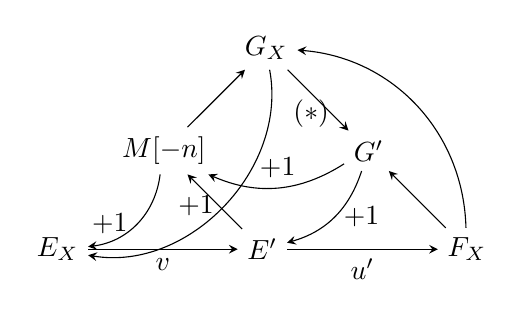
\begin{tikzpicture}[>=stealth,baseline=(GX.base),node distance=1.0cm]
  \node (EX) at (0,0) {$E_X$};
  \node (Ep) at (2.6,0) {$E'$};
  \node (FX) at (5.2,0) {$F_X$};
  \node (M)  at (1.35,1.25) {$M[-n]$};
  \node (GX) at (2.65,2.55) {$G_X$};
  \node (Gp) at (3.95,1.25) {$G'$};
  \node at (3.22,1.72) {$(*)$};
  \draw[->] (EX) -- node[below] {$v$} (Ep);
  \draw[->] (Ep) -- node[below] {$u'$} (FX);
  \draw[->] (Ep) -- (M);
  \draw[->] (M) -- (GX);
  \draw[->] (GX) -- (Gp);
  \draw[->] (FX) -- (Gp);
  \draw[->] (M) to[bend left=38] node[left] {$+1$} (EX);
  \draw[->] (Gp) to[bend left=28] node[above] {$+1$} (M);
  \draw[->] (Gp) to[bend left=28] node[right] {$+1$} (Ep);
  \draw[->] (GX) to[bend left=55] node[left] {$+1$} (EX);
  \draw[->] (FX) to[bend right=42] (GX);
\end{tikzpicture}
\]
八面体中标出的特异三角的上同调正合列表明
\[
  \Ho^n(G_X)\longrightarrow \Ho^n(G')
\]
为满态射; 因此 \(\Ho^n(G')\) 确实为 \(\mathcal C_0\)-有限型.

所以, 上述修正将问题归结到 \(\Ho^{n+1}(u)\) 为单态射的情形. 以下作此假设. 于是 \(E\to F\to G\) 的上同调正合列给出正合列
\[
  \Ho^n(E)\xrightarrow{\Ho^n(u)}
  \Ho^n(F)\longrightarrow \Ho^n(G)\longrightarrow 0.
\]
由于 \(\Ho^n(G)\) 为 \(\mathcal C_0\)-有限型, 在 \(S\) 上满足存在满态射
\[
  M\longrightarrow \Ho^n(G_X),\qquad M\in\Ob\mathcal C_{0,X},
\]
的 \(X\) 的集合, 按定义是 \(S\) 的加细. 利用 \(\mathcal C_0\) 在 \(\mathcal C\) 中的拟可提升性, 可要求此满态射经由 \(Z^n(F_X)\) 分解:
\[
  M\xrightarrow{s}Z^n(F_X)\longrightarrow \Ho^n(F_X)\longrightarrow \Ho^n(G_X).
\]
显然, 取 \(r=0\), 如 \hyperlink{sga6.e01.prop.1-4-1}{(1.4.1)} 中定义的 \(u'\) 是复形态射, 并且
\[
  \Ho^n(u'):\Ho^n(E_X)\oplus M\longrightarrow \Ho^n(F_X)
\]
为满态射. 这就完成了 \hyperlink{sga6.e01.prop.1-4-1}{(1.4.1)} 的证明.

\sgaStableTarget{sga6.e01.lem.1-4-2}\textbf{引理 1.4.2.} 设 \(\mathcal C\) 为 Abel 范畴, \(u:E\to F\) 为 \(\mathcal C\) 中的复形态射 (相应地, \(\Dpx(\mathcal C)\) 中的箭头), \(G\) 为 \(u\) 的锥. 对给定的 \(n\in\mathbb Z\), 下列条件等价:
\begin{enumerate}[label=(\roman*)]
\item 对 \(i\geq n\), 有 \(\Ho^i(G)=0\);
\item \(\Ho^i(u)\) 在 \(i>n\) 时为同构, 在 \(i=n\) 时为满态射.
\end{enumerate}
证明由上同调正合列立即得出.

\sgaStableTarget{sga6.e01.def.1-4-3}\textbf{定义 1.4.3.} 若 \(u\) 满足 \hyperlink{sga6.e01.lem.1-4-2}{(1.4.2)} 中的等价条件, 则称 \(u\) 为 \(n\)-\emph{拟同构} (相应地, \(n\)-\emph{同构}).

于是由 \hyperlink{sga6.e01.prop.1-4-1}{(1.4.1)} 立即推出:

\sgaStableTarget{sga6.e01.cor.1-4-4}\textbf{推论 1.4.4.} 设 \(S,S,\mathcal C,\mathcal C_0\) 如 \hyperlink{sga6.e01.prop.1-4-1}{(1.4.1)}. 固定 \(n\in\mathbb Z\), 设 \(u:E\to F\) 为 \(\mathcal C_S\) 中复形的 \((n+1)\)-拟同构, 且 \(\Ho^n(G)\) 为 \(\mathcal C_0\)-有限型. 则在 \(S\) 上满足存在如 \hyperlink{sga6.e01.prop.1-4-1}{(1.4.1)} 中的 \((M,r,s)\), 使 \(u'\) 为 \(n\)-拟同构的 \(X\) 的集合, 是 \(S\) 的加细.

形象地说, 利用 \(\Ho^n(G)\) 的有限性条件, 可在局部“前进一步”: 在 \(E^n\) 上添加一个 \(\mathcal C_0\) 中的对象, 从而局部改变 \(u\) 在次数 \(n\) 处的部分, 使 \(u\) 成为 \(n\)-拟同构.

\sgaStableTarget{sga6.e01.cor.1-4-5}\textbf{推论 1.4.5.} 设 \(\mathcal C\) 为 Abel 范畴, \(n\in\mathbb Z\), \(u:E\to F\) 为 \(\mathcal C\) 中复形的 \(n\)-拟同构. 则 \(\Cpx(\mathcal C)\) 中存在交换图
\[
\begin{tikzcd}
E \arrow[r,"v"] \arrow[d,"u"'] & E' \arrow[dl,"u'"]\\
F &
\end{tikzcd}
\]
其中 \(u'\) 为拟同构, \(v\) 为单态射, 并在次数 \(\geq n\) 处诱导恒等, 即
\[
  E'^i=E^i,\qquad v^i=\id(E^i)\qquad\text{当 }i\geq n.
\]

\emph{证明.} 在 \(S\) 为单点景、\(\mathcal C_0=\mathcal C\) 的情形应用 \hyperlink{sga6.e01.cor.1-4-4}{(1.4.4)}, 得到 \(\Cpx(\mathcal C)\) 中的交换三角
\[
\begin{tikzcd}
E \arrow[r,"v_{n-1}"] \arrow[d,"u"'] & E'_{\,n-1} \arrow[dl,"u'_{n-1}"]\\
F &
\end{tikzcd}
\]
其中 \(u'_{n-1}\) 是 \((n-1)\)-拟同构, \(v_{n-1}\) 为在次数 \(\geq n\) 处诱导恒等的单态射. 重复这一过程, 对 \(i\leq n-1\), 得到 \(\Cpx(\mathcal C)\) 中一列交换三角
\[
\begin{tikzcd}
E'_i \arrow[r,"v_{i-1}"] \arrow[d,"u'_i"'] & E'_{\,i-1} \arrow[dl,"u'_{i-1}"]\\
F &
\end{tikzcd}
\]
其中 \(u'_i\) 是 \(i\)-拟同构, \(v_{i-1}\) 是在次数 \(\geq i\) 处诱导恒等的单态射. 取极限即得推论. 更确切地, 用 \(d'_i\) 表示 \(E'_i\) 的微分, 定义 \(E'\) 如下:
\[
  E'^i=E^i,\quad d'^i=d^i\quad (i\geq n),
\]
以及
\[
  E'^i=(E'_i)^i,\quad d'^i=(d'_i)^i\quad (i<n),
\]
再定义 \(v\) 和 \(u'\) 为
\[
  v^j=(v_i)^j,\qquad u'^j=(u'_i)^j\qquad (i\leq j).
\]
立即可验证这样定义的 \(E'\)、\(v\) 和 \(u'\) 满足要求.

简言之, 可以将一个 \(n\)-拟同构延拓为拟同构, 而“不改变在次数 \(>n\) 处给定的任何内容”.

\sgaStableTarget{sga6.e01.sec.2}\section*{2. 伪凝聚复形}

\sgaStableTarget{sga6.e01.para.2-0}\textbf{2.0.} 本节中, \(S\) 表示景, \(S\) 表示 \(S\) 的一个对象, \(\mathcal C\) 表示平坦 Abel \(S\)-范畴 \hyperlink{sga6.e01.sec.1.1}{(1.1)}, \(\mathcal C_0\) 表示 \(\mathcal C\) 的严格满加性子 \(S\)-范畴. 假设 \(\mathcal C_0\) 局部对满态射的核拟稳定 \hyperlink{sga6.e01.sec.1.2}{(1.2)}, 且在 \(\mathcal C\) 中局部拟可提升 \hyperlink{sga6.e01.sec.1.2}{(1.2)}.

\sgaStableTarget{sga6.e01.def.2-1}\textbf{定义 2.1.} 设 \(X\in\Ob S\), \(E\) 为 \(\mathcal C_X\) 中的复形, \(n\in\mathbb Z\). 若对充分大的 \(i\), 有 \(E^i=0\), 且对 \(i\geq n\) (相应地, 对每个 \(i\); 相应地, 对每个 \(i\), 并且除有限多个 \(i\) 外均有 \(E^i=0\)) 有 \(E^i\in\Ob\mathcal C_{0,S}\), 则称 \(E\) 为\emph{严格 \(\mathcal C_0\)-\(n\)-伪凝聚} (相应地, 严格 \(\mathcal C_0\)-伪凝聚; 相应地, 严格 \(\mathcal C_0\)-完美) 复形.

不致混淆时, 有时将“严格 \(\mathcal C_0\)-\(n\)-伪凝聚”简称为“严格 \(n\)-伪凝聚” (其余术语亦然).

\sgaStableTarget{sga6.e01.lem.2-1-1}\textbf{引理 2.1.1.} 设 \(E\in\Ob\Cpx(\mathcal C_S)\), \(n\in\mathbb Z\). 若 \(E\) 严格 \(n\)-伪凝聚, 且对 \(i>n\) 有 \(\Ho^i(E)=0\), 则 \(\Ho^n(E)\) 有限型.

\emph{证明.} 序列
\[
  0\longrightarrow Z^n(E)\longrightarrow E^n\longrightarrow E^{n+1}\longrightarrow\cdots\longrightarrow 0
\]
正合, 且对 \(i\geq n\), 有 \(E^i\in\Ob\mathcal C_0\). 由于 \(\mathcal C_0\) 局部对满态射的核拟稳定, \(Z^n(E)\) 有限型, 从而作为它的商的 \(\Ho^n(E)\) 也有限型.

\sgaStableTarget{sga6.e01.prop.2-2}\textbf{命题 2.2.} 设 \(F\in\Ob\Dpx(\mathcal C_S)\), \(n\in\mathbb Z\). 则:

\textbf{a)} 若 \(F\) 严格 \(n\)-伪凝聚 (相对于 \(\mathcal C_0\)), 且
\[
  u:E\longrightarrow F
\]
为拟同构, 则在 \(S\) 上满足存在拟同构
\[
  v:F'\longrightarrow E_X
\]
且 \(F'\) 严格 \(n\)-伪凝聚的 \(X\) 的集合, 是 \(S\) 的加细.

\textbf{b)} 下列条件等价:
\begin{enumerate}[label=(\roman*)]
\item 在 \(S\) 上满足存在 \(\Cpx(\mathcal C_X)\) 中的拟同构
\[
  u:E\longrightarrow F_X
\]
且 \(E\) 严格 \(n\)-伪凝聚的 \(X\) 的集合, 是 \(S\) 的加细;
\item[\((\mathrm{i}')\)] 与 (i) 相同的条件, 但把 \(u\) 换成 \(\Dpx(\mathcal C_X)\) 中的同构;
\item 在 \(S\) 上满足存在 \(\Cpx(\mathcal C_X)\) 中的 \(n\)-拟同构
\[
  u:E\longrightarrow F_X
\]
且 \(E\) 严格完美的 \(X\) 的集合, 是 \(S\) 的加细;
\item[\((\mathrm{ii}')\)] 与 (ii) 相同的条件, 但把 \(u\) 换成 \(\Dpx(\mathcal C_X)\) 中的 \(n\)-同构.
\end{enumerate}

\emph{证明.} 对于 a), 当 \(i\) 充分大时, 存在 \(i\)-拟同构
\[
  v_i:F'_i\longrightarrow E
\]
其中 \(F'_i\) 严格 \(n\)-伪凝聚 (取 \(F'_i=0\)). 我们证明, 若 \(i>n\), 则在加细 \(S\) 后, 存在 \((i-1)\)-拟同构
\[
  v_{i-1}:F'_{i-1}\longrightarrow E
\]
其中 \(F'_{i-1}\) 严格 \(n\)-伪凝聚. 由 \hyperlink{sga6.e01.cor.1-4-4}{(1.4.4)}, 只需证明 \(\Ho^{i-1}(M')\) 为 \(\mathcal C_0\)-有限型, 这里 \(M'\) 是 \(v_i\) 的锥. 现若用 \(M''\) 表示 \(uv_i\) 的锥, 由 \(u\) 为拟同构的假设和 \hyperlink{sga6.e01.lem.1-4-2}{(1.4.2)} 可得
\[
  \Ho^j(M')\qis \Ho^j(M'')\qquad\text{对所有 }j,
\]
以及
\[
  \Ho^j(M')=0\qquad\text{当 }j\geq i.
\]
另一方面, 锥的公式
\[
  M''{}^j=F'_i{}^{\,j+1}\oplus F^j
\]
表明 \(M''\) 严格 \((i-1)\)-伪凝聚. 因而由 \hyperlink{sga6.e01.lem.2-1-1}{(2.1.1)},
\[
  \Ho^{i-1}(M'')=\Ho^{i-1}(M')
\]
有限型, 断言得证. 反复应用这一过程, 并在加细 \(S\) 后, 可得 \(n\)-拟同构
\[
  v_n:F'_n\longrightarrow E
\]
其中 \(F'_n\) 严格 \(n\)-伪凝聚. 然而由 \hyperlink{sga6.e01.cor.1-4-5}{(1.4.5)}, 可以把 \(v_n\) 延拓为拟同构
\[
  v:F'\longrightarrow E
\]
而不改变次数 \(\geq n\) 处的任何内容; 特别地, \(F'\) 严格 \(n\)-伪凝聚. 这就证明了 a).

对于 b), (i) 与 \((\mathrm{i}')\) 的等价性, 由 a) 及 \(\Dpx^-(\mathcal C_X)\) 中同构的定义立即得出. 若 \(E\in\Ob\Dpx^-(\mathcal C_S)\) 严格 \(n\)-伪凝聚, 则有正合列
\[
  0\longrightarrow E'\longrightarrow E\longrightarrow E''\longrightarrow 0
\]
其中 \(E'\) 严格完美, 且对 \(i\geq n\), 有 \(E''{}^i=0\). 所以 \(E'\to E\) 为 \(n\)-拟同构, 得到蕴涵 \((\mathrm{i})\Rightarrow(\mathrm{ii})\). 蕴涵 \((\mathrm{ii})\Rightarrow(\mathrm{ii}')\) 是平凡的, 因此只需证明 \((\mathrm{ii}')\Rightarrow(\mathrm{i})\). 设
\[
  u:E\longrightarrow F
\]
为 \(\Dpx^-(\mathcal C_S)\) 中的 \(n\)-同构, 其中 \(E\) 严格完美. 则 \(u\) 可由 \(\Cpx^-(\mathcal C_S)\) 中的一个图表示
\[
\begin{tikzcd}
& E' \arrow[dl,"s"'] \arrow[dr,"u'"]\\
E && F ,
\end{tikzcd}
\]
其中 \(s\) 为拟同构, \(u'\) 为 \(n\)-拟同构. 由 a), 加细 \(S\) 后, 存在拟同构
\[
  t:E''\longrightarrow E',
\]
其中 \(E''\) 严格 \(n\)-伪凝聚. 对 \(u't:E''\to F\) 应用 \hyperlink{sga6.e01.cor.1-4-5}{(1.4.5)}, 将其延拓为拟同构
\[
  E'''\longrightarrow F
\]
其中 \(E'''\) 严格 \(n\)-伪凝聚. 这就证明了 \((\mathrm{ii}')\Rightarrow(\mathrm{i})\), 并完成了 \hyperlink{sga6.e01.prop.2-2}{(2.2)} 的证明.

\sgaStableTarget{sga6.e01.def.2-3}\textbf{定义 2.3.} 在 \hyperlink{sga6.e01.prop.2-2}{(2.2)} 的假设下, 若 \(F\in\Ob\Dpx^-(\mathcal C_S)\) 满足 \hyperlink{sga6.e01.prop.2-2}{(2.2)} b) 中的等价条件, 就称 \(F\) 为 \(n\)-\(\mathcal C_0\)-伪凝聚复形. 若 \(F\) 对每个 \(n\) 都是 \(n\)-\(\mathcal C_0\)-伪凝聚的, 就称 \(F\) 为 \(\mathcal C_0\)-伪凝聚复形.

不致混淆时, 有时把 \(n\)-\(\mathcal C_0\)-伪凝聚、\(\mathcal C_0\)-伪凝聚分别简称为 \(n\)-伪凝聚、伪凝聚.

\sgaStableTarget{sga6.e01.rem.2-3-1}\textbf{注 2.3.1.} 设 \(F\in\Ob\Dpx(\mathcal C_S)\) 为伪凝聚复形. 在 \(S\) 上满足存在拟同构
\[
  E\longrightarrow F_X
\]
且 \(E\) 严格伪凝聚 \hyperlink{sga6.e01.def.2-1}{(2.1)} 的 \(X\) 的集合, 一般不是 \(S\) 的加细. 不过后面 (\hyperlink{sga6.e01.prop.2-7}{2.7} a) 及\hyperlink{sga6.e02.expose}{第 II 讲}) 将看到此结论成立的若干重要情形.

(\hyperlink{sga6.e01.prop.2-2}{2.2} a) 的证明给出下述结果.

\sgaStableTarget{sga6.e01.prop.2-4}\textbf{命题 2.4.} 设 \(n,i\in\mathbb Z\),
\[
  u:E\longrightarrow F
\]
为 \(\Cpx(\mathcal C_S)\) 中的 \(i\)-拟同构, 其中 \(F\) 为 \(n\)-伪凝聚复形, \(E\) 为严格 \(n\)-伪凝聚复形. 则加细 \(S\) 后, 在 \(\Cpx(\mathcal C_S)\) 中存在交换三角
\[
\begin{tikzcd}
E \arrow[r,"v"] \arrow[d,"u"'] & E' \arrow[dl,"u'"]\\
F &
\end{tikzcd}
\]
其中 \(E'\) 严格 \(n\)-伪凝聚, \(u'\) 为拟同构, \(v\) 为在次数 \(\geq i\) 处诱导恒等的单态射.

\sgaStableTarget{sga6.e01.prop.2-5}\textbf{命题 2.5.} \textbf{a)} 若 \(F\in\Ob\Dpx(\mathcal C_S)\) 是 \(n\)-伪凝聚 (相应地, 伪凝聚) 的, 则 \(F[m]\) 是 \((n-m)\)-伪凝聚 (相应地, 伪凝聚) 的.

\textbf{b)} 设
\sgaStableTarget{sga6.e01.eq.unnamed.occ2}\[
\begin{tikzcd}
E \arrow[rr] && F \arrow[dl]\\
& G \arrow[ul,"+1"] &
\end{tikzcd}
\tag{*}
\]
为 \(\Dpx(\mathcal C_S)\) 中的特异三角. 若 \(E\) 和 \(G\) 均为 \(n\)-伪凝聚 (相应地, 伪凝聚) 的, 则 \(F\) 为 \(n\)-伪凝聚 (相应地, 伪凝聚) 的.

\emph{证明.} a) 由定义是平凡的.

b) 当然只需证明非括号中的断言. 三角 \((*)\) 也可写为
\[
\begin{tikzcd}
G[-1] \arrow[rr] && E \arrow[dl]\\
& F \arrow[ul,"+1"] &
\end{tikzcd}
\]
由 a), \(G[-1]\) 为 \((n+1)\)-伪凝聚复形. 因而只需证明: 若 \(E\) 为 \((n+1)\)-伪凝聚复形, \(F\) 为 \(n\)-伪凝聚复形, 则 \(G\) 为 \(n\)-伪凝聚复形. 局部化后, 可设 \(E\) (相应地, \(F\)) 严格 \((n+1)\)-伪凝聚 (相应地, 严格 \(n\)-伪凝聚). \(\Dpx^-(\mathcal C_S)\) 中的箭头
\[
  E\xrightarrow{u}F
\]
可由 \(\Cpx^-(\mathcal C_S)\) 中的一对箭头表示
\[
\begin{tikzcd}
& E' \arrow[dl,"s"'] \arrow[dr,"u'"]\\
E && F ,
\end{tikzcd}
\]
其中 \(s\) 为拟同构. 由 (\hyperlink{sga6.e01.prop.2-2}{2.2} a)), 局部化后存在拟同构
\[
  t:E''\longrightarrow E',
\]
其中 \(E''\) 严格 \((n+1)\)-伪凝聚. 因而归结到 \(u\) 由 \(\Cpx^-(\mathcal C_S)\) 中真正的箭头定义的情形. 此时断言由定义及公式
\[
  C(u)^i=E^{i+1}\oplus F^i,
\]
得出, 这里 \(C(u)\) 表示 \(u\) 的锥.

\sgaStableTarget{sga6.e01.schol.2-6}\textbf{说明 2.6.} 通过三角的旋转可见, 三角 \((*)\) 中两个对象的伪凝聚性质, 蕴涵第三个对象的某种伪凝聚性质. 各种情形可归纳在下表中; 小写字母表示伪凝聚的次数, 每行中加下划线者为结论:
\[
\begin{array}{ccc}
E&F&G\\[0.2em]
n+1&n&\underline n\\
n&\underline n&n\\
\underline n&n&n-1 .
\end{array}
\]

用
\[
  \Dpx(\mathcal C)_{\mathcal C_0\text{-}n\mathrm{coh}}
  \quad\text{相应地}\quad
  \Dpx(\mathcal C)_{\mathcal C_0\text{-}\mathrm{coh}}
\]
表示 \(\Dpx(\mathcal C)\) 的严格满纤维子范畴, 其在每个 \(X\in\Ob S\) 上的纤维由 \(\Dpx(\mathcal C_X)\) 中相对于 \(\mathcal C_0\) 为 \(n\)-伪凝聚 (相应地, 伪凝聚) 的对象组成. 由 \hyperlink{sga6.e01.prop.2-5}{(2.5)}, 范畴
\[
  \Dpx(\mathcal C)_{\mathcal C_0\text{-}\mathrm{coh}}
\]
是 \(\Dpx(\mathcal C)\) 的三角子 \(S\)-范畴 \hyperlink{sga6.e01.sec.1.1}{(1.1)}.

\sgaStableTarget{sga6.e01.prop.2-7}\textbf{命题 2.7.} 假设 \(S\) 为单点景, 因而
\[
  \mathcal C=\mathcal C_S,\qquad \mathcal C_0=\mathcal C_{0,S}.
\]
则:
\begin{enumerate}[label=\alph*)]
\item 若 \(F\in\Ob\Dpx(\mathcal C)\) 伪凝聚, 则存在拟同构
\[
  E\longrightarrow F
\]
其中 \(E\) 严格伪凝聚 \hyperlink{sga6.e01.def.2-1}{(2.1)}.
\item 用 \(\Kpx^{-,\mathrm{ac}}(\mathcal C_0)\) 表示 \(\Kpx^-(\mathcal C_0)\) 中由无上同调复形构成的满三角子范畴. 典范函子
\[
  \Kpx^-(\mathcal C_0)/\Kpx^{-,\mathrm{ac}}(\mathcal C_0)
  \longrightarrow \Dpx(\mathcal C)
\]
完全忠实, 其本质像为 \(\Dpx(\mathcal C)_{\mathcal C_0\text{-}\mathrm{coh}}\).
\end{enumerate}

\emph{证明.} a) 设 \(F\in\Ob\Dpx(\mathcal C)_{\mathcal C_0\text{-}\mathrm{coh}}\), 并假设已构造出 \(\Cpx(\mathcal C)\) 中的 \(i\)-拟同构
\[
  u_i:E_i\longrightarrow F
\]
其中 \(E_i\) 严格伪凝聚; 当 \(i\) 充分大时, 取 \(E_i=0\) 即可. 设 \(G_i\) 为 \(u_i\) 的锥. 由 \hyperlink{sga6.e01.lem.1-4-2}{(1.4.2)} 和 \hyperlink{sga6.e01.lem.2-1-1}{(2.1.1)}, \(\Ho^{i-1}(G_i)\) 为 \(\mathcal C_0\)-有限型. 所以由 \hyperlink{sga6.e01.cor.1-4-4}{(1.4.4)}, \(\Cpx(\mathcal C)\) 中存在交换三角
\[
\begin{tikzcd}
E_i \arrow[r,"v_{i-1}"] \arrow[d,"u_i"'] & E_{i-1} \arrow[dl,"u_{i-1}"]\\
F &
\end{tikzcd}
\]
其中 \(E_{i-1}\) 严格伪凝聚, \(u_{i-1}\) 为 \((i-1)\)-拟同构, \(v_{i-1}\) 为在次数 \(\geq i\) 处诱导恒等的单态射. 取极限 (参见 \hyperlink{sga6.e01.cor.1-4-5}{(1.4.5)} 的证明), 得到拟同构
\[
  u:E\longrightarrow F
\]
其中 \(E\) 严格伪凝聚.

b) 将 \([V]\), 第 I 章第 2 节, 4.2 b)(i) 的判据与 a) 结合应用.

注意到 a) 的证明还给出以下更精确的结果, 它推广了 \hyperlink{sga6.e01.cor.1-4-5}{(1.4.5)}.

\sgaStableTarget{sga6.e01.prop.2-7-1}\textbf{命题 2.7.1.} 在 \hyperlink{sga6.e01.prop.2-7}{(2.7)} 的假设下, 设 \(u:E\to F\) 为 \(\Cpx(\mathcal C)\) 中的 \(n\)-拟同构, 其中 \(F\) 伪凝聚, \(E\) 严格伪凝聚. 则 \(\Cpx(\mathcal C)\) 中存在交换三角
\[
\begin{tikzcd}
E \arrow[r,"v"] \arrow[d,"u"'] & E' \arrow[dl,"u'"]\\
F &
\end{tikzcd}
\]
其中 \(E'\) 严格伪凝聚, \(u'\) 为拟同构, \(v\) 为在次数 \(\geq n\) 处诱导恒等的单态射.

\sgaStableTarget{sga6.e01.def.2-8}\textbf{定义 2.8.} 设 \(n\in\mathbb N\), \(F\in\Ob\mathcal C_S\). 若在 \(S\) 上满足存在正合列
\[
  E^{-n}\longrightarrow\cdots\longrightarrow E^0\longrightarrow F_X\longrightarrow 0,
\qquad E^i\in\Ob\mathcal C_{0,X}\quad(-n\leq i\leq 0),
\]
的 \(X\) 的集合是 \(S\) 的加细, 则称 \(F\) 为 \(n\)-\(\mathcal C_0\)-有限表示的. 若 \(F\) 对每个 \(n\in\mathbb N\) 都是 \(n\)-\(\mathcal C_0\)-有限表示的, 则称 \(F\) 为 \(\infty\)-\(\mathcal C_0\)-有限表示的.

当然, 当 \(\mathcal C_0\) 不致引起歧义时, 有时简称 \(n\)-有限表示. 将“1-有限表示”称为“有限表示”, 将“0-有限表示”称为“有限型”; 后一概念与 \hyperlink{sga6.e01.sec.1.2}{(1.2)} 中已引入的概念相同.

\sgaStableTarget{sga6.e01.prop.2-9}\textbf{命题 2.9.} 设 \(n\in\mathbb N\), \(F\in\Ob\mathcal C_S\). 下列条件等价:
\begin{enumerate}[label=(\roman*)]
\item \(F\) 为 \(n\)-有限表示 (相应地, \(\infty\)-有限表示) 的;
\item \(F\) 为 \((-n)\)-伪凝聚 (相应地, 伪凝聚) 的.
\end{enumerate}
在 \(S\) 为单点景的情形, \(F\) 伪凝聚的充要条件是存在正合列
\[
  \cdots\longrightarrow E^i\longrightarrow\cdots\longrightarrow E^0\longrightarrow F\longrightarrow 0,
\qquad E^i\in\Ob\mathcal C_0\quad\text{对所有 }i.
\]

\emph{证明.} 对于等价性 \((\mathrm{i})\Leftrightarrow(\mathrm{ii})\), 显然只需处理非括号中的情形. 蕴涵 \((\mathrm{i})\Rightarrow(\mathrm{ii})\) 由定义立即得出, 而 \((\mathrm{ii})\Rightarrow(\mathrm{i})\) 由 \hyperlink{sga6.e01.prop.2-4}{(2.4)} 立即得出: 箭头 \(0\to F\) 是 \(1\)-拟同构, 因而局部化后得到拟同构
\[
  E\longrightarrow F
\]
其中 \(E\) 严格 \((-n)\)-伪凝聚, 且对 \(i\geq 1\), 有 \(E^i=0\), 即得 \(F\) 的一个 \(n\)-有限表示. 第二个断言同样用 \hyperlink{sga6.e01.prop.2-7-1}{(2.7.1)} 证明.

\sgaStableTarget{sga6.e01.prop.2-10}\textbf{命题 2.10.} \textbf{a)} 设 \(m,n\in\mathbb Z\), \(n\leq m\). 若 \(F\in\Ob\Dpx^-(\mathcal C_S)\) 是 \(n\)-伪凝聚复形, 且在次数 \(\geq m\) 处无上同调, 则局部存在拟同构
\[
  E\longrightarrow F
\]
其中 \(E\) 严格 \(n\)-伪凝聚, 且对 \(i\geq m\), 有 \(E^i=0\). 若 \(S\) 为单点景, 且 \(F\) 伪凝聚并在次数 \(\geq m\) 处无上同调, 则存在拟同构
\[
  E\longrightarrow F
\]
其中 \(E\) 严格伪凝聚, 且对 \(i\geq m\), 有 \(E^i=0\).

\textbf{b)} 设 \(F\in\Ob\Dpx^-(\mathcal C_S)\) 在次数 \(>n\) 处无上同调. \(F\) 为 \(n\)-伪凝聚的充要条件是 \(\Ho^n(F)\) 有限型.

\emph{证明.} a) 由于 \(F\) 在次数 \(\geq m\) 处无上同调, 箭头 \(0\to F\) 是 \(m\)-拟同构. 断言由 \hyperlink{sga6.e01.prop.2-4}{(2.4)} 和 \hyperlink{sga6.e01.prop.2-7-1}{(2.7.1)} 得出.

b) 在 \(\Dpx^-(\mathcal C_S)\) 中存在特异三角:
\[
\begin{tikzcd}
F \arrow[rr] && F' \arrow[dl]\\
& \Ho^n(F)[-n] \arrow[ul,"+1"] &
\end{tikzcd}
\]
(为看出这一点, 先截断 \(F\), 将 \(F^n\) 换成 \(Z^n(F)\), 并对 \(i>n\) 将 \(F^i\) 换成 \(0\)). 上同调正合列给出
\[
  \Ho^i(F')=0\quad\text{当 }i\geq n-1,
\]
所以 \(F'\) 为 \((n-1)\)-伪凝聚复形. 由 \hyperlink{sga6.e01.prop.2-5}{(2.5)} 和 \hyperlink{sga6.e01.schol.2-6}{(2.6)} 即得结论.



% Additional notation for Expose I continuation
\providecommand{\RHom}{\mathrm R\!\Hom}
\providecommand{\Ext}{\operatorname{Ext}}
\providecommand{\coh}{\operatorname{coh}}
\providecommand{\PreCoh}{\operatorname{precoh}}
\providecommand{\Tr}{\operatorname{Tr}}
\providecommand{\Qis}{\operatorname{Qis}}
\providecommand{\Rad}{\operatorname{rad}}
\providecommand{\Spec}{\operatorname{Spec}}
\providecommand{\End}{\operatorname{End}}
\providecommand{\Id}{\operatorname{Id}}
\providecommand{\varinjlim}{\mathop{\mathrm{lim}}\limits_{\longrightarrow}}
\providecommand{\varprojlim}{\mathop{\mathrm{lim}}\limits_{\longleftarrow}}
\providecommand{\qcoh}{\operatorname{qcoh}}
\providecommand{\amp}{\operatorname{amp}}


\sgaStableTarget{sga6.e01.expose.occ2}\section*{第 I 讲 (续): 伪凝聚复形与完美复形}

\sgaStableTarget{sga6.e01.prop.2-11}\textbf{命题 2.11.} 设 \(n\in\mathbb Z\).

\textbf{a)} 设 \(F\in\Ob\Cpx^-(\mathcal C_S)\). 若对每个 \(i\geq n\) (相应地, 每个 \(i\)), \(F^i\) 为 \((i-n)\)-有限表示 (相应地, \(\infty\)-有限表示) 的, 则 \(F\) 为 \(n\)-伪凝聚 (相应地, 伪凝聚) 的.

\textbf{b)} 设 \(F\in\Ob\Dpx^-(\mathcal C_S)\). 若对每个 \(i\geq n\) (相应地, 每个 \(i\)), \(\Ho^i(F)\) 为 \((i-n)\)-有限表示 (相应地, \(\infty\)-有限表示) 的, 则 \(F\) 伪凝聚.

\emph{证明.} 只需处理非括号中的断言.

\textbf{a)} 对满足 \(F^i\neq0\) 只可能发生在 \(i\leq n+N\) 的 \(N\) 作归纳. 若 \(N=0\), 断言由 (\hyperlink{sga6.e01.prop.2-10}{2.10} b) 立即得出. 设 \(N\geq1\). 有正合列
\[
  0\longrightarrow F^{n+N}[-n-N]\longrightarrow F\longrightarrow F'\longrightarrow 0 .
\]
由归纳假设, \(F'\) 为 \(n\)-伪凝聚复形; 另一方面, 由假设和 (\hyperlink{sga6.e01.prop.2-9}{2.9} 及 \hyperlink{sga6.e01.prop.2-5}{2.5} a), \(F^{n+N}[-n-N]\) 为 \(n\)-伪凝聚复形. 因而由 (\hyperlink{sga6.e01.prop.2-5}{2.5} b), \(F\) 为 \(n\)-伪凝聚复形.

\textbf{b)} 对满足 \(\Ho^i(F)=0\) 当 \(i>n+N\) 的 \(N\) 作归纳. 若 \(N=0\), 断言由 (\hyperlink{sga6.e01.prop.2-10}{2.10} b) 得出. 设 \(N\geq1\). 如同 (\hyperlink{sga6.e01.prop.2-10}{2.10} b) 的证明, 在 \(\Dpx^-(\mathcal C_S)\) 中有特异三角
\[
  F'\longrightarrow F\longrightarrow \Ho^{n+N}(F)[-n-N]\longrightarrow F'[1].
\]
更明确地说, 其锥为 \(\Ho^{n+N}(F)[-n-N]\). 上同调正合列给出
\[
  \Ho^i(F')=0\quad\text{当 } i>n+N-1,
\]
即当 \(i>(n-1)+(N-1)\), 以及
\[
  \Ho^i(F')\qis \Ho^{i+1}(F)\quad\text{当 }i<n+N-1 .
\]
所以由归纳假设 (用 \(n-1\) 代替 \(n\)), \(F'\) 为 \((n-1)\)-伪凝聚复形. 另一方面, 由 (\hyperlink{sga6.e01.prop.2-9}{2.9} 及 \hyperlink{sga6.e01.prop.2-5}{2.5} a), \(\Ho^{n+N}(F)[-n-N]\) 为 \(n\)-伪凝聚复形. 所以由 \hyperlink{sga6.e01.schol.2-6}{(2.6)}, \(F\) 为 \(n\)-伪凝聚复形.

\sgaStableTarget{sga6.e01.rem.2-11-1}\textbf{注 2.11.1.} 若 \(F\) 伪凝聚, 则各 \(F^i\) (相应地, 各 \(\Ho^i(F)\)) 一般不伪凝聚, 甚至不一定有限型. 不过, 在下一节关于凝聚性概念的讨论中, 将看到一些重要例子, 其中 \(F\) 的伪凝聚性蕴涵各 \(\Ho^i(F)\) 的伪凝聚性.

\sgaStableTarget{sga6.e01.prop.2-12}\textbf{命题 2.12.} 设 \(F',F''\in\Ob\Dpx^-(\mathcal C_S)\), \(F=F'\oplus F''\). \(F\) 为 \(n\)-伪凝聚 (相应地, 伪凝聚) 的充要条件, 是 \(F'
\) 和 \(F''\) 均为 \(n\)-伪凝聚 (相应地, 伪凝聚) 的.

\emph{证明.} 只需证明非括号中的断言. 充分性显然; 下面证明必要性. 由归纳法, 可设已经证明了 \(F'\) 和 \(F''\) 均为 \((n+1)\)-伪凝聚的. 局部化后, 甚至可设 \(F'\) 与 \(F''\) 都严格 \((n+1)\)-伪凝聚, 且在 \(\Cpx^-(\mathcal C_S)\) 中有 \(F=F'\oplus F''\). 用 \(F'_{>n}\) (相应地, \(F'_{\leq n}\)) 表示把 \(F'\) 中 \(i\leq n\) (相应地, \(i>n\)) 处的 \(F'^i\) 换成 \(0\) 得到的复形; 类似地定义 \(F''_{>n}\) 和 \(F''_{\leq n}\). 有正合列
\[
  0\longrightarrow F'_{>n}\oplus F''_{>n}\longrightarrow F
  \longrightarrow F'_{\leq n}\oplus F''_{\leq n}\longrightarrow 0 .
\]
复形 \(F'_{>n}\oplus F''_{>n}\) 严格完美; 由于 \(F\) 是 \(n\)-伪凝聚的, 由 \hyperlink{sga6.e01.schol.2-6}{(2.6)}, \(F'_{\leq n}\oplus F''_{\leq n}\) 为 \(n\)-伪凝聚复形. 由 (\hyperlink{sga6.e01.prop.2-10}{2.10} b), 这意味着
\[
  \Ho^n(F'_{\leq n}\oplus F''_{\leq n})
\]
有限型. 然而
\[
  \Ho^n(F'_{\leq n}\oplus F''_{\leq n})
  =\Ho^n(F'_{\leq n})\oplus \Ho^n(F''_{\leq n}),
\]
所以 \(\Ho^n(F'_{\leq n})\) (相应地, \(\Ho^n(F''_{\leq n})\)) 有限型; 再次由 (\hyperlink{sga6.e01.prop.2-10}{2.10} b), \(F'_{\leq n}\) (相应地, \(F''_{\leq n}\)) 为 \(n\)-伪凝聚复形. 将 \hyperlink{sga6.e01.prop.2-5}{(2.5)} 应用于正合列
\[
  0\longrightarrow F'_{>n}\longrightarrow F'\longrightarrow F'_{\leq n}\longrightarrow 0
\]
(对 \(F''\) 同样处理), 可得 \(F'\) 与 \(F''\) 均为 \(n\)-伪凝聚的.

\sgaStableTarget{sga6.e01.prop.2-13}\textbf{命题 2.13.} 设三元组 \((S',\mathcal C',\mathcal C'_0)\) 与 \((S,\mathcal C,\mathcal C_0)\) 满足相同的假设 \hyperlink{sga6.e01.para.2-0}{(2.0)}. 设 \(f:S'\to S\) 为景的态射, 对应的底层函子为 \(f^{-1}:S\to S'\), 又设
\[
  u:\Dpx^*(\mathcal C)\longrightarrow \Dpx^*(\mathcal C')\qquad (*=+,-,b)
\]
为 \(f\) 之上的 Cartesian 函子, 且在每个纤维上正合. 假设存在 \(a,b\in\mathbb Z\), 使对每个 \(S\in\Ob S\) 均满足下列条件:

\begin{enumerate}[label=(\roman*)]
\item 若 \(E\in\Ob\mathcal C_{0,S}\), 则 \(u(E)\) 为 \(a\)-\(\mathcal C'_0\)-伪凝聚 (相应地, \(\mathcal C'_0\)-伪凝聚) 的;
\item 若 \(F\in\Ob\Dpx^*(\mathcal C_S)\) 在次数 \(>0\) 处无上同调, 则 \(u(F)\) 在次数 \(>b\) 处无上同调.
\end{enumerate}

则若 \(F\in\Ob\Dpx^*(\mathcal C_S)\) 相对于 \(\mathcal C_0\) 为 \(m\)-伪凝聚的, 且在次数 \(>n\) 处无上同调, 对象
\[
  u(F)\in\Ob\Dpx^*(\mathcal C'_{S'}),\qquad S'=f^{-1}(S),
\]
相对于 \(\mathcal C'_0\) 为 \(\sup(m+b,n+a)\)-伪凝聚 (相应地, \((m+b)\)-伪凝聚) 的, 且在次数 \(>n+b\) 处无上同调. 特别地, 在括号中的情形, 若 \(F\in\Ob\Dpx^*(\mathcal C_S)\) 相对于 \(\mathcal C_0\) 伪凝聚, 则 \(u(F)\) 相对于 \(\mathcal C'_0\) 伪凝聚.

\emph{证明.} 只需考虑非括号中的情形. 先设 \(F\in\Ob\Dpx^*(\mathcal C_S)\) 严格完美 \hyperlink{sga6.e01.def.2-1}{(2.1)}, 且当 \(i>n\) 时 \(F^i=0\). 则 \(u(F)\) 为 \((n+a)\)-\(\mathcal C'_0\)-伪凝聚复形. 对满足 \(F^i\neq0\) 的指标 \(i\) 的个数 \(N\) 作归纳. 若 \(N=1\), 则对某个 \(p\leq n\), 有 \(F=F^p[-p]\), 所以 \(u(F)\) 为 \((p+a)\)-\(\mathcal C'_0\)-伪凝聚复形, 从而更是 \((n+a)\)-伪凝聚复形. 若 \(N>1\), 则有正合列
\[
  0\longrightarrow F'\longrightarrow F\longrightarrow F''\longrightarrow 0,
\]
其中 \(F'\) 与 \(F''\) 为长度 \(<N-1\) 的严格完美复形, 且对 \(i>n\) 有 \(F'^i=F''^i=0\). 对特异三角
\[
  u(F')\longrightarrow u(F)\longrightarrow u(F'')\longrightarrow u(F')[1].
\]
应用 (\hyperlink{sga6.e01.prop.2-5}{2.5} b), 并利用归纳假设, 得到 \(u(F)\) 为 \((n+a)\)-伪凝聚复形.

现转到一般情形: \(F\) 为 \(m\)-\(\mathcal C_0\)-伪凝聚复形, 且在次数 \(>n\) 处无上同调. 局部化后, 由 (\hyperlink{sga6.e01.prop.2-10}{2.10} a), 可设 \(F\) 严格 \(m\)-伪凝聚, 且对 \(i>n\) 有 \(F^i=0\). 于是有正合列
\[
  0\longrightarrow F'\longrightarrow F\longrightarrow F''\longrightarrow 0,
\]
其中 \(F''\) 在次数 \(\geq m\) 处为零, 而 \(F'\) 严格完美且在次数 \(>n\) 处为零. 在特异三角
\[
  u(F')\longrightarrow u(F)\longrightarrow u(F'')\longrightarrow u(F')[1].
\]
中, 对象 \(u(F'')\) 在次数 \(>m+b\) 处无上同调, 因而为 \((m+b)\)-伪凝聚的, 而由刚才的证明, \(u(F')\) 为 \((n+a)\)-伪凝聚的. 由 (\hyperlink{sga6.e01.prop.2-5}{2.5} b) 即得结论.

\sgaStableTarget{sga6.e01.cor.2-14}\textbf{推论 2.14.} 设 \(\mathcal C_1\) 为 \(\mathcal C\) 的严格满加性子 \(S\)-范畴, 满足
\[
  \mathcal C_0\subset \mathcal C_1\subset \mathcal C.
\]
假设 \(\mathcal C_1\) 的每个对象都为 \(\mathcal C_0\)-伪凝聚的. 则:

\begin{enumerate}[label=(\roman*)]
\item \(\mathcal C_1\) 在 \(\mathcal C\) 中局部拟可提升 \hyperlink{sga6.e01.sec.1.2}{(1.2)}, 且局部对满态射的核拟稳定 \hyperlink{sga6.e01.sec.1.2}{(1.2)};
\item 对 \(S\in\Ob S\) 及 \(F\in\Ob\Dpx(\mathcal C_S)\), \(F\) 相对于 \(\mathcal C_1\) 为 \(n\)-伪凝聚 (相应地, 伪凝聚) 的充要条件, 是它相对于 \(\mathcal C_0\) 具有同一性质.
\end{enumerate}

\emph{证明.} 对于 (i), 设 \(E\to F\) 为 \(\mathcal C_S\) 中的满态射, 其中 \(F\in\Ob\mathcal C_{1,S}\). 由于 \(F\) 为 \(\mathcal C_0\)-伪凝聚的, 从而更是 \(\mathcal C_0\)-有限型的, 局部化后存在满态射 \(E'\to F\), 其中 \(E'\in\Ob\mathcal C_{0,S}\). 利用 \(\mathcal C_0\) 在 \(\mathcal C\) 中的拟可提升性, 再次局部化后, 可设该满态射经由 \(E\) 分解; 这就得到 \(\mathcal C_1\) 的拟可提升性. 另一方面, 若 \(E\in\Ob\mathcal C_S\) 具有由 \(\mathcal C_1\) 的对象组成的有限右消解, 则由 (\hyperlink{sga6.e01.prop.2-11}{2.11} a), \(E\) 为 \(\mathcal C_0\)-伪凝聚的, 从而更是 \(\mathcal C_1\)-有限型的.

对于 (ii), 只需证明必要性. 为此, 可任选 (\hyperlink{sga6.e01.prop.2-11}{2.11} a) 或 \hyperlink{sga6.e01.prop.2-13}{(2.13)} 来应用, 取 \(S'=S\)、\(\mathcal C'=\mathcal C\)、\(f=\Id\)、\(u=\Id\), 并将 \(\mathcal C'_0\) 与 \(\mathcal C_0\) 分别换成 \(\mathcal C_0\) 和 \(\mathcal C_1\).

\sgaStableTarget{sga6.e01.schol.2-14-1}\textbf{说明 2.14.1.} 因此, 存在 \(\mathcal C\) 的一个最大的严格满加性子 \(S\)-范畴, 它给出与 \(\mathcal C_0\) 相同的 \(n\)-伪凝聚性 (相应地, 伪凝聚性) 概念; 这就是由 \(\mathcal C_0\)-伪凝聚对象构成的范畴. 后一个范畴局部对满态射的核稳定.

\sgaStableTarget{sga6.e01.ex.2-15}\textbf{例 2.15.} 设 \((S,A)\) 为赋环拓扑斯, \(\mathcal C,\mathcal C_0\) 为 (\hyperlink{sga6.e01.sec.1.3}{1.3} d) 中考虑的 \(S\)-范畴. 纤维范畴 \(\Dpx(\mathcal C)\) 常记为 \(\Dpx(S,A)\), 或在要强调模为左 \(A\)-模时记为 \(\Dpx_A(S)\), 若 \(A\) 不致引起歧义, 甚至简称为 \(\Dpx(S)\). 用 \(S\) 表示 \(S\) 的终对象, 并令 \(\Dpx(\mathcal C_S)=\Dpx_A(S)\) (或 \(\Dpx(S)\)). 若 \(\Dpx(S)\) 的对象为 \(n\)-\(\mathcal C_0\)-伪凝聚 (相应地, \(\mathcal C_0\)-伪凝聚) 的, 就称它为 \(n\)-伪凝聚 (相应地, 伪凝聚) 的; 严格的概念也采用同样约定. 在 \hyperlink{sga6.e01.schol.2-6}{(2.6)} 中记为 \(\Dpx(\mathcal C)_{n-\mathcal C_0-\coh}\) (相应地, \(\Dpx(\mathcal C)_{\mathcal C_0-\coh}\)) 的 \(\Dpx(\mathcal C)\) 的纤维子范畴, 将记为 \(\Dpx_A(S)_{n-\coh}\) (相应地, \(\Dpx_A(S)_{\coh}\)). 注意到由 \hyperlink{sga6.e01.cor.2-14}{(2.14)}, 将 \(\mathcal C_0\) 换成如下定义的 \(S\)-范畴 \(\mathcal C_1\), 得到相同的伪凝聚性概念:
\[
  U\longmapsto \text{局部为有限型自由模直和因子的左 }A_U\text{-模所成的范畴}.
\]
若一个 \(A\)-模 \(M\) 是有限型自由 \(A\)-模的直和因子, 一般不能推出 \(M\) 局部自由有限型. 不过有下述结果.

\sgaStableTarget{sga6.e01.lem.2-15-1}\textbf{引理 2.15.1.} 假设 \(S\) 满足下列两个假设之一:
\begin{enumerate}[label=(\roman*)]
\item \(S\) 有足够多的点 (SGA 4 IV 6.4), 且对 \(S\) 的每个点 \(s\), 有限型投射左 \(A_s\)-模均自由; 例如, 若 \(A_s/\Rad(A_s)\) 为域, 或 \(\Rad(A_s)\) 幂零, 就满足后一条件;
\item \((S,A)\) 是 [1] 意义下的“局部赋环”拓扑斯, 即 \(A\) 交换, 且对每个 \(X\in\Ob S\) 及每个 \(f\in\Gamma(X,A)\), 有
\[
  X=X_f\cup X_{1-f},
\]
其中 \(X_f\) (相应地, \(X_{1-f}\)) 表示 \(X\) 上使 \(f\) (相应地, \(1-f\)) 可逆的最大子对象.
\end{enumerate}
则每个有限型自由左 \(A\)-模的直和因子, 都是有限型局部自由模.

\emph{证明.} 先假设 (i) 成立. 注意到, 若 \(E\) 和 \(F\) 为两个 \(A\)-模, 且 \(E\) 有限表示, 则对 \(S\) 的每个点 \(s\), 典范箭头
\[
  \Hom(E,F)_s\longrightarrow \Hom(E_s,F_s)
\]
是同构. 因此, 若 \(E\) 与 \(F\) 都有限表示, 且在 \(S\) 的某点 \(s\) 有 \(E_s\qis F_s\), 则存在 \(S\) 的一个带 \(s\)-点的对象 \(U\), 使 \(E|U\qis F|U\). 结论立即得出.

再假设 (ii) 成立. 设 \(n\in\mathbb N\), 用 \(\mathbb D^n\) 表示在属于某个固定宇宙的局部赋环拓扑斯的范畴上, 由下式定义的函子
\[
  T\longmapsto \Gamma(T,\mathcal O_T)^n.
\]
已知 [1], 函子 \(\End_{\mathbb D}(\mathbb D^n)\) 由
\[
  M_n=\Spec\mathbb Z[T_{ij}]\quad(1\leq i\leq n,
  1\leq j\leq n),
\]
连同由矩阵 \((T_{ij})\) 定义的 \((\mathcal O_{M_n})^n\) 的自同态 \(U_n\) 所表示. 现设
\[
  p:A^n\longrightarrow A^n
\]
为投影子. 下面证明 \(p(A^n)\) 局部自由有限型. 由上述结果, 存在局部赋环拓扑斯的态射
\[
  s:S\longrightarrow M_n
\]
使 \(s^*(u_n)=p\). 可以把 \(s\) 解释为 \(M_n\) 的一个取值于 \(\Gamma(S,A)\) 的点, 即一个系数在 \(\Gamma(S,A)\) 中的 \(n\) 阶矩阵. 由于该矩阵是投影子, \(s\) 经由闭子概形
\[
  i:P_n\hookrightarrow M_n
\]
分解; 记为 \(S\xrightarrow{s'}P_n\xrightarrow{i}M_n\). 因而
\[
  p=s'^* i^*(u_n),
\]
于是证明完毕, 因为由假设 (i) 下的断言, \(i^*(u_n)\) 的像是有限型局部自由层.

\sgaStableTarget{sga6.e01.cor.2-16}\textbf{推论 2.16.} 设
\[
  f:(S',A')\longrightarrow (S,A)
\]
为赋环拓扑斯的态射, 由函子 \(f^{-1}:S\to S'\) 及环层态射 \(f^{-1}(A)\to A'\) 定义. 用 \(\Dpx(_{A'}S'_A)\) 表示 \(A'\)-\(A\)-双模的导出范畴, 其中 \(A'\) 从左作用、\(A\) 从右作用, 并设
\[
  \otimes_A^{\mathrm L}:\Dpx^-(_{A'}S'_A)\times_{S'}\Dpx^-(_A S)
  \longrightarrow \Dpx^-(_{A'}S')
\]
为张量积
\[
  (E',E)\longmapsto E'\otimes_A f^{-1}(E).
\]
的导出函子. 设 \(X\in\Ob S\), 令 \(X'=u(X)\), 又设 \(E'\in\Ob\Dpx^-(_{A'}X'_A)\)、\(E\in\Ob\Dpx^-(_A X)\). 若 \(E'\) 为 \(m'\)-伪凝聚的 (视为 \(\Dpx^-(_A S')\) 中的对象), 且在次数 \(>n'\) 处无上同调, 而 \(E\) 为 \(m\)-伪凝聚的, 且在次数 \(>n\) 处无上同调, 则
\[
  E'\otimes_A^{\mathrm L}E
\]
为 \(\sup(m+n',m'+n)\)-伪凝聚的, 且在次数 \(>n+n'\) 处无上同调.

\emph{证明.} 将 \(S\) 换成 \(S/X\), 可设 \(X=S\); 在 \hyperlink{sga6.e01.prop.2-13}{(2.13)} 中取
\[
  u=E'\otimes_A^{\mathrm L}:\Dpx^-(_A S)\longrightarrow \Dpx^-(_{A'}S').
\]
设 \(U\in\Ob S\)、\(U'=f^{-1}(U)\), \(E\) 为左 \(A_U\)-模的复形. 若 \(E\) 在次数 \(>n\) 处无上同调, 则由 \(\otimes_A^{\mathrm L}\) 的定义, \(E'\otimes_A^{\mathrm L}E\) 在次数 \(>n+n'\) 处无上同调. 另一方面, 若 \(E=(A_U)^p\), 则
\[
  E'\otimes_A^{\mathrm L}E=(E'|U')^p,
\]
由假设和 \hyperlink{sga6.e01.prop.2-12}{(2.12)}, 它为 \(m'\)-伪凝聚的. 因此 \hyperlink{sga6.e01.prop.2-13}{(2.13)} 的条件满足, 其中 \(a=m'\)、\(b=n'\), 结论得证.

特别地:

\sgaStableTarget{sga6.e01.cor.2-16-1}\textbf{推论 2.16.1.} 在 \hyperlink{sga6.e01.cor.2-16}{(2.16)} 的假设下, 有:

\textbf{a)} 函子
\[
  \mathrm L f^*: \Dpx^-(_A S)\longrightarrow \Dpx^-(_{A'}S')
\]
(它就是函子 \(A'\otimes_A^{\mathrm L}\)) 诱导函子
\[
  \mathrm L f^*: \Dpx^-(_A S)_{\coh}\longrightarrow \Dpx^-(_{A'}S')_{\coh}
\]
(采用 \hyperlink{sga6.e01.schol.2-6}{(2.6)} 中的记号).

\textbf{b)} 若 \(A\) 交换, 则函子
\[
  \otimes_A^{\mathrm L}:\Dpx^-(S)\times_S\Dpx^-(S)
  \longrightarrow \Dpx^-(S)
\]
诱导函子
\[
  \otimes_A^{\mathrm L}:\Dpx^-(S)_{\coh}\times_S\Dpx^-(S)_{\coh}
  \longrightarrow \Dpx^-(S)_{\coh} .
\]

\sgaStableTarget{sga6.e01.exercise.2-16-2}\textbf{习题 2.16.2.} 设 \(S\) 为拓扑斯, \(A\to A'\) 为 \(S\) 中的环态射. 假设满足下列条件之一:
\begin{enumerate}[label=(\roman*)]
\item \(A\to A'\) 满射, 且其核为幂零理想;
\item 左 \(A\)-模范畴上的函子 \(A'\otimes_A-\) 正合且忠实.
\end{enumerate}
证明 \(E\in\Ob\Dpx^-(_A S)\) 为 \(n\)-伪凝聚 (相应地, 伪凝聚) 的充要条件是
\[
  A'\otimes_A E\in\Ob\Dpx^-(_{A'}S)
\]
为 \(n\)-伪凝聚 (相应地, 伪凝聚) 的.

提示: 先证明左 \(A\)-模 \(L\) 有限型, 当且仅当 \(A'\otimes_A L\) 有限型 (参见 Bourbaki, \emph{Commutative Algebra}, 第 I 章第 3 节命题 11, 及第 II 章第 3 节命题 4), 再利用 \hyperlink{sga6.e01.prop.2-5}{(2.5)} 和 (\hyperlink{sga6.e01.prop.2-10}{2.10} b), 通过截断归结到这一情形.

\sgaStableTarget{sga6.e01.sec.3}\section*{3. 与经典凝聚性概念的联系}

\sgaStableTarget{sga6.e01.para.3-0}\textbf{3.0.} 假设和记号与 \hyperlink{sga6.e01.para.2-0}{(2.0)} 相同, 但不再假设 \(\mathcal C_0\) 局部对满态射的核拟稳定.

\sgaStableTarget{sga6.e01.def.3-1}\textbf{定义 3.1.} 设 \(F\in\Ob\mathcal C_S\). 若对 \(S\) 上每个 \(U\) 及每个态射
\[
  u:E\longrightarrow F|U,
\]
其中 \(E\in\Ob\mathcal C_{0,U}\), \(\Ker(u)\) 都为 \(\mathcal C_0\)-有限型 \hyperlink{sga6.e01.sec.1.2}{(1.2)}, 则称 \(F\) 相对于 \(\mathcal C_0\) \emph{预凝聚} (precoherent). 若 \(F\) 预凝聚且有限型, 则称 \(F\) 相对于 \(\mathcal C_0\) \emph{凝聚}.

\emph{技术说明.} 这里引入预凝聚概念仅作为技术性的中间环节; 需要记住的只有凝聚性概念.

\sgaStableTarget{sga6.e01.rem.3-2}\textbf{注 3.2.} 设 \(F\in\Ob\mathcal C_S\). 由定义显然可知, 若 \(F\) 预凝聚 (相应地, 有限型), 则 \(F\) 的每个子对象 (相应地, 商对象) 也预凝聚 (相应地, 有限型).

\sgaStableTarget{sga6.e01.lem.3-3}\textbf{引理 3.3.}

\textbf{a)} 设
\[
  0\longrightarrow F\longrightarrow G\longrightarrow H
\]
为 \(\mathcal C_S\) 中的正合列. 若 \(G\) 有限型, \(H\) 预凝聚, 则 \(F\) 有限型.

\textbf{b)} 设
\[
  F\longrightarrow G\longrightarrow H\longrightarrow 0
\]
为 \(\mathcal C_S\) 中的正合列. 若 \(F\) 有限型, \(G\) 预凝聚, 则 \(H\) 预凝聚.

\textbf{c)} 设
\[
  0\longrightarrow F\longrightarrow G\longrightarrow H\longrightarrow 0
\]
为 \(\mathcal C_S\) 中的正合列. 若 \(F\) 与 \(H\) 预凝聚 (相应地, 有限型), 则 \(G\) 也有同一性质.

\emph{证明.} a) 局部化后, 存在满态射 \(G'\to G\), 其中 \(G'\in\Ob\mathcal C_0\). 因而有行正合的交换图
\[
\begin{tikzcd}
0\arrow[r]&F'\arrow[r]\arrow[d]&G'\arrow[r]\arrow[d]&H\arrow[d,"\Id"]\\
0\arrow[r]&F\arrow[r]&G\arrow[r]&H .
\end{tikzcd}
\]
由于 \(H\) 预凝聚, \(F'\) 有限型; 然而 \(F'\to F\) 为满态射, 所以 \(F\) 有限型.

b) 设 \(U\) 在 \(S\) 上, \(H'\xrightarrow{f}H|U\) 为 \(\mathcal C_U\) 中的态射, 其中 \(H'\in\Ob\mathcal C_{0,U}\). 改换记号后, 可设 \(U=S\). 由 \(\mathcal C_0\) 在 \(\mathcal C\) 中的拟可提升性, 局部化后存在交换方块
\[
\begin{tikzcd}
G' \arrow[r,"p"] \arrow[d] & H' \arrow[d,"f"]\\
G \arrow[r] & H,
\end{tikzcd}
\]
其中水平箭头为满态射, 且 \(G'\in\Ob\mathcal C_0\). 由于 \(\Ker(f)\) 是 \(\Ker(fp)\) 的商, 只需证明 \(\Ker(fp)\) 有限型; 因而可设 \(H'=G'\). 箭头 \(F\to G\) 及 \(H'\to G\) 定义了
\[
  g:F\oplus H'\longrightarrow G.
\]
令 \(K=\Ker(G\to H)\), 得到行正合且 \(q\) 为满态射的交换图
\[
\begin{tikzcd}
0\arrow[r]&F\arrow[r]\arrow[d,"q"]&F\oplus H'\arrow[r]\arrow[d,"g"]&H'\arrow[r]\arrow[d,"f"]&0\\
0\arrow[r]&K\arrow[r]&G\arrow[r]&H\arrow[r]&0 .
\end{tikzcd}
\]
由蛇形图可知 \(\Ker(g)\to\Ker(f)\) 为满态射. 然而, 由于 \(F\oplus H'\) 有限型, \(G\) 预凝聚, 由 a) 得 \(\Ker(g)\) 有限型; 结论得证.

c) 先证明非括号中的断言. 改换记号后, 只需证明: 若 \(g:G'\to G\) 为 \(\mathcal C_S\) 中的态射, 且 \(G'\in\Ob\mathcal C_0\), 则 \(\Ker(g)\) 有限型. 设 \(H'\) 为复合箭头 \(G'\to H\) 的像. 有行正合的交换图
\[
\begin{tikzcd}
0\arrow[r]&F'\arrow[r]\arrow[d,"f"]&G'\arrow[r]\arrow[d,"g"]&H'\arrow[r]\arrow[d,"h"]&0\\
0\arrow[r]&F\arrow[r]&G\arrow[r]&H\arrow[r]&0 .
\end{tikzcd}
\]
由于 \(h\) 为单态射, 蛇形图给出同构 \(\Ker(f)\qis\Ker(g)\). 然而由 a), \(F'\) 有限型; 再由 a), \(\Ker(f)\) 有限型. 这就证明了非括号中的断言. 对于括号中的断言, 严格说来不能引用 (\hyperlink{sga6.e01.prop.2-5}{2.5} b), 因为未假设 \(\mathcal C_0\) 局部对满态射的核拟稳定. 局部化后, 有满态射
\[
  F'\xrightarrow{u}F,
  \qquad H'\xrightarrow{v}H,
\]
其中 \(F',H'\in\Ob\mathcal C_0\). 再次局部化后, 可设 \(v\) 经由 \(G\) 分解, 因而有行正合的交换图
\[
\begin{tikzcd}
0\arrow[r]&F'\arrow[r]\arrow[d,"u"]&F'\oplus H'\arrow[r]\arrow[d,"w"]&H'\arrow[r]\arrow[d,"v"]&0\\
0\arrow[r]&F\arrow[r]&G\arrow[r]&H\arrow[r]&0 .
\end{tikzcd}
\]
由于 \(u\) 与 \(v\) 都是满态射, \(w\) 也为满态射, 断言得证. \hyperlink{sga6.e01.lem.3-3}{(3.3)} 证明完毕.

立即得到:

\sgaStableTarget{sga6.e01.cor.3-4}\textbf{推论 3.4.} \(\mathcal C_S\) 中由凝聚对象构成的满 (相应地, 严格满) 子范畴, 在有限射影 (相应地, 归纳) 极限下稳定. 特别地, 两个凝聚对象之间箭头的核、余核及像都凝聚. 设
\[
  E^0\longrightarrow E^1\longrightarrow E^2\longrightarrow E^3\longrightarrow E^4
\]
为 \(\mathcal C_S\) 中的正合列. 若 \(E^0,E^1,E^3,E^4\) 均凝聚, 则 \(E^2\) 也凝聚.

\sgaStableTarget{sga6.e01.cor.3-5}\textbf{推论 3.5.} 假设 \(\mathcal C_0\) 的对象均为 \(\mathcal C_0\)-凝聚的 (这特别蕴涵 \(\mathcal C_0\) 局部对满态射的核拟稳定, 即满足 \hyperlink{sga6.e01.para.2-0}{(2.0)} 的条件).

\textbf{a)} 对 \(F\in\Ob\mathcal C_S\), 下列条件等价:
\begin{enumerate}[label=(\roman*)]
\item \(F\) 有限表示;
\item \(F\) 凝聚;
\item \(F\) 为 \(\infty\)-有限表示的 \hyperlink{sga6.e01.def.2-8}{(2.8)}.
\end{enumerate}

\textbf{b)} 设 \(F\in\Ob\Dpx^-(\mathcal C_S)\), \(n\in\mathbb Z\). 则
\[
\begin{split}
F\text{ 为 }n\text{-伪凝聚复形}
\quad\Longleftrightarrow\quad&
\Ho^i(F)\text{ 对 }i\geq n+1\text{ 均凝聚},\\
&\text{且 }\Ho^n(F)\text{ 有限型.}
\end{split}
\]
特别地, \(F\) 伪凝聚的充要条件是对每个 \(n\), \(\Ho^n(F)\) 都凝聚.

\emph{证明.} 断言 a) 与 b) 中的蕴涵 \(\Rightarrow\), 由 \hyperlink{sga6.e01.cor.3-4}{(3.4)} 平凡地得出. b) 中的蕴涵 \(\Leftarrow\) 由 a) 和 (\hyperlink{sga6.e01.prop.2-11}{2.11} b) 立即得出.

\sgaStableTarget{sga6.e01.ex.3-6}\textbf{例 3.6.} 设 \((S,A)\) 为赋环拓扑斯, \(\mathcal C,\mathcal C_0\) 为 (\hyperlink{sga6.e01.sec.1.3}{1.3} d) 中的 \(S\)-范畴, 亦如 \hyperlink{sga6.e01.ex.2-15}{(2.15)}. \(\mathcal C_0\) 的对象都凝聚的充要条件是 \(A\) 凝聚, 即预凝聚. 下面是满足此条件的例子:
\begin{itemize}
\item \(A\) 为以左 Noether 环为值的常值环 (SGA 4 IX 2.1);
\item \(S\) 为局部 Noether 概形 \(S\) 上 Zariski 拓扑的集合层拓扑斯, 且 \(A=\mathcal O_S\);
\item \(S\) 为复解析空间 \(S\) 上集合层的拓扑斯, 且 \(A=\mathcal O_S\).
\end{itemize}
另一方面, 拓扑空间上的复值连续函数层一般不凝聚.

当然, 若 \((S,A)\) 由赋环空间定义, 则这里的凝聚性概念与 Serre 的通常概念相同 (EGA \(0_I\), 5.3.1).

\sgaStableTarget{sga6.e01.prop.3-7}\textbf{命题 3.7.} \textbf{a)} 设
\[
  f:(S',A')\longrightarrow(S,A)
\]
为赋环拓扑斯的态射. 假设 \(f\) 右平坦, 即函子 \(f^*=A'\otimes_A-\) 正合. 对 \(F\in\Ob\Dpx_A^-(S)\) 及 \(G\in\Ob\Dpx_A^+(S)\), 存在函子性的典范箭头
\[
  f^*\RHom(F,G)\longrightarrow \RHom(f^*(F),f^*(G)).
\]
当 \(F\) 伪凝聚时, 这个箭头是同构.

\textbf{b)} 假设 \(A\) 交换且凝聚, 又设 \(F\in\Ob\Dpx^-(S)\)、\(G\in\Ob\Dpx^+(S)\). 若对所有 \(i\), \(\Ho^i(F)\) 和 \(\Ho^i(G)\) 都凝聚, 则 \(\Ext^i(F,G)\) 也都凝聚.

\emph{证明.} a) 为定义此箭头 (参见 SGA 4 XVII), 可设 \(G\) 的各分量为内射对象, 然后取复合箭头
\[
  f^*\Hom(F,G)\longrightarrow \Hom(f^*F,f^*G)
  \longrightarrow \RHom(f^*F,f^*G).
\]
下面证明, 当 \(F\) 伪凝聚时它是同构. 为简便, 用 \(T\) (相应地, \(T'\)) 表示函子 \(f^*\RHom(\cdot,G)\) (相应地, \(\RHom(f^*\cdot,f^*G)\)), 取 \(a\in\mathbb Z\), 使当 \(i<a\) 时 \(\Ho^i(G)=0\). 显然有 \(TA\qis T'A\), 因而由分解论证, 对严格完美的 \(F\) \hyperlink{sga6.e01.def.2-1}{(2.1)}, 有 \(TF\qis T'F\). 另一方面, 若 \(F\) 在次数 \(>n\) 处无上同调, 则 \(TF\) 和 \(T'F\) 在次数 \(<a-n\) 处无上同调. 为验证伪凝聚的 \(F\) 满足 \(TF\qis T'F\), 由于问题是局部的, 可设 \(F\) 严格 \(n\)-伪凝聚; 即存在特异三角
\[
  F'\longrightarrow F\longrightarrow F''\longrightarrow F'[1].
\]
其中 \(F'\) 严格完美, \(F''\) 在次数 \(>n-1\) 处无上同调. 由此得到特异三角之间的态射
\[
\begin{tikzcd}[column sep=tiny]
TF'' \arrow[r] \arrow[d] & TF \arrow[r] \arrow[d] & TF' \arrow[d] \\
T'F'' \arrow[r] & T'F \arrow[r] & T'F' .
\end{tikzcd}
\]
由于 \(F'\) 严格完美, 有 \(TF'\qis T'F'\); 而 \(TF''\) 及 \(T'F''\) 在次数 \(\leq a-n\) 处无上同调. 写出上述三角的上同调正合列之间所诱导的态射, 可得 \(TF\to T'F\) 对 \(i\leq a-n\) 诱导同构
\[
  \Ho^i(TF)\qis \Ho^i(T'F)
\]
. 由于 \(n\) 可以取得任意小, 断言得证.

b) 证明留给读者作为习题; 例如参见 [H] II 3.3.

\sgaStableTarget{sga6.e01.rem.3-7-1}\textbf{注 3.7.1.} 后面 \hyperlink{sga6.e01.prop.7-1-2}{(7.1.2)} 将看到 \(\RHom\) 与 \(\mathrm L f^*\) 相容的另一个情形.

\sgaStableTarget{sga6.e01.cor.3-7-2}\textbf{推论 3.7.2.} (参见 EGA \(0_I\), 5.2.7.) 设 \((S,A)\) 为赋环拓扑斯, \(s\) 为 \(S\) 的一个点 (SGA 4 VIII 7.8), 又设
\[
  E,F\in\Ob\D^b_{A,\coh}(S).
\]
若 \(E_s\qis F_s\), 则存在 \(S\) 的一个带 \(s\)-点的对象 \(U\), 使
\[
  E|U\qis F|U.
\]

\emph{证明.} 设 \(\alpha:E_s\to F_s\) 及 \(\beta:F_s\to E_s\) 为互逆同构. 由 (\hyperlink{sga6.e01.prop.3-7}{2.22} a), 有
\[
  \Hom(E,F)_s\qis\Hom(E_s,F_s),
  \qquad
  \Hom(F,E)_s\qis\Hom(F_s,E_s).
\]
因此存在 \(s\) 的邻域 \(U\) 及 \(\Hom(E,F)\) (相应地, \(\Hom(F,E)\)) 在 \(U\) 上的截面 \(u\) (相应地, \(v\)), 使 \(u_s=\alpha\) (相应地, \(v_s=\beta\)). 态射 \(vu:E|U\to E|U\) 及 \(uv:F|U\to F|U\) 在 \(s\) 处诱导恒等; 因而在 \(U\) 上某个适当的 \(V\) 上也是恒等, 如所欲证.

\sgaStableTarget{sga6.e01.sec.4}\section*{4. 完美复形}

\sgaStableTarget{sga6.e01.para.4-0}\textbf{4.0.} 本节中, \(S\) 表示景, \(S\) 表示 \(S\) 的一个对象, \(\mathcal C\) 表示平坦 Abel \(S\)-范畴, \(\mathcal C_0\) 表示 \(\mathcal C\) 的严格满加性子 \(S\)-范畴 \hyperlink{sga6.e01.sec.1.1}{(1.1)}. 除非另有说明, 假设 \(\mathcal C_0\) 在 \(\mathcal C\) 中局部可提升, 且局部对满态射的核稳定 \hyperlink{sga6.e01.sec.1.2}{(1.2)}.

\sgaStableTarget{sga6.e01.lem.4-1}\textbf{引理 4.1.} 设
\[
  u:E\longrightarrow F
\]
为 \(\Cpx(\mathcal C_S)\) 中的箭头. 若 \(E\) 严格 \(\mathcal C_0\)-完美 \hyperlink{sga6.e01.def.2-1}{(2.1)}, 且 \(F\) 无上同调, 则 \(u\) 局部同伦于零.

\emph{证明.} 需要局部构造同伦 \(k\), 使
\[
  u=dk+kd.
\]
由于 \(E\) 严格完美, 存在 \(a,b\in\mathbb Z\), \(a\leq b\), 使当 \(i\notin[a,b]\) 时 \(E^i=0\). 所以对 \(i\notin[a,b]\), 可取 \(k^i=0\). 对 \(i>a\), 按 \(i\) 递减归纳构造 \(k^i\). 假设已构造 \(k^i:E^i\to F^{i-1}\), 使对 \(i>n>a\) 有
\[
  u^i=k^{i+1}d_E^i+d_F^{i-1}k^i
\]
. 我们证明, 局部化后存在
\[
  k^{n-1}:E^{n-1}\longrightarrow F^{n-2}
\]
使
\[
  u^{n-1}=k^n d_E^{n-1}+d_F^{n-2}k^{n-1}.
\]
由归纳假设, 箭头
\[
  v^{n-1}=u^{n-1}-k^n d_E^{n-1}:E^{n-1}\longrightarrow F^{n-1}
\]
经由 \(Z^{n-1}(F)\) 分解. 然而 \(F\) 无上同调, 所以 \(Z^{n-1}(F)=B^{n-1}(F)\). 由于 \(\mathcal C_0\) 在 \(\mathcal C\) 中局部可提升, 局部化后存在 \(k^{n-1}:E^{n-1}\to F^{n-2}\), 使 \(v^{n-1}=d_F^{n-2}k^{n-1}\), 如所欲证.

\sgaStableTarget{sga6.e01.cor.4-2}\textbf{推论 4.2.} 设
\[
\begin{tikzcd}
P \arrow[d,"v"'] \\
F & E \arrow[l,"f"]
\end{tikzcd}
\]
为 \(\Cpx(\mathcal C_S)\) 中的图, 其中 \(P\) 严格 \(\mathcal C_0\)-完美, \(f\) 为拟同构. 在 \(S\) 上满足存在 \(\Cpx(\mathcal C_X)\) 中的箭头
\[
  u:P_X\longrightarrow E_X
\]
使图
\[
\begin{tikzcd}
& P_X \arrow[d,"v_X"]\\
E_X \arrow[r,"f_X"'] \arrow[ur,"u"] & F_X
\end{tikzcd}
\]
在 \(\Kpx(\mathcal C_X)\) 中交换的 \(X\) 的集合, 是 \(S\) 的加细.

\emph{证明.} 设 \(G\) 为 \(f\) 的锥. 有正合列
\[
  \longrightarrow \Hom_{\Kpx(\mathcal C_S)}(P,E)
  \longrightarrow \Hom_{\Kpx(\mathcal C_S)}(P,F)
  \longrightarrow \Hom_{\Kpx(\mathcal C_S)}(P,G)
  \longrightarrow .
\]
由于 \(G\) 无上同调, 由 \hyperlink{sga6.e01.lem.4-1}{(4.1)}, \(v\) 在 \(\Hom_{\Kpx(\mathcal C_S)}(P,G)\) 中的像局部为零. 因此局部化后存在 \(u:P\to E\), 使在 \(\Kpx(\mathcal C_S)\) 中有 \(v=fu\), 如所欲证.

\sgaStableTarget{sga6.e01.cor.4-3}\textbf{推论 4.3.} 设 \(f:E\to F\) 为 \(\Cpx(\mathcal C_S)\) 中的拟同构, 其中 \(F\) 相对于 \(\mathcal C_0\) 严格完美. 在 \(S\) 上满足存在拟同构
\[
  g:F_X\longrightarrow E_X
\]
且 \(f_Xg\) 同伦于 \(\Id_{F_X}\) 的 \(X\) 的集合, 是 \(S\) 的加细.

\emph{证明.} 这是 \hyperlink{sga6.e01.cor.4-2}{(4.2)} 的特殊情形.

\sgaStableTarget{sga6.e01.schol.4-4}\textbf{说明 4.4.} 设 \(F\in\Ob\Kpx(\mathcal C_S)\). 例如, 借助 \(\mathcal C\) 的一个劈裂 (SGA 1 VI 7.1), 可定义在 \(S/S\) 上纤维化的范畴 \((\Qis/F)\), 它在 \(S\) 上每个 \(X\) 处的纤维, 为以 \(F_X\) 为靶的拟同构所成范畴的对偶范畴 \((\Qis/F_X)^\circ\). 于是 \hyperlink{sga6.e01.cor.4-3}{(4.3)} 可以表述为: 若 \(F\) 严格完美, 则箭头 \(\Id_F\) 在 \((\Qis/F)\) 中局部共尾.

